\documentclass{llncs}

\usepackage{paralist}

\usepackage{amssymb, amsmath}
\usepackage{enumitem}
\usepackage{todonotes}
\usepackage{subcaption}
\captionsetup{compatibility=false}
\usepackage{url}
\usepackage{graphicx}
\usepackage{xcolor}
%\usepackage{rotating}
\usepackage{tikz}
\graphicspath{{figures/}}
\usetikzlibrary{calc,trees,positioning,arrows,chains,automata,shapes.geometric,%
    decorations.pathreplacing,decorations.pathmorphing,shapes,%
    matrix,shapes.symbols}

\usetikzlibrary{shapes,arrows,automata,positioning,calc}
\usetikzlibrary{fit,backgrounds}
\usetikzlibrary{decorations.pathreplacing}
\tikzset{
>=stealth',
  punktchain/.style={
    rectangle,
    rounded corners,
    % fill=black!10,
    draw=black, very thick,
    text width=6em,
    minimum height=3em,
    text centered,
    on chain},
  line/.style={draw, thick, <-},
  element/.style={
    tape,
    top color=white,
    bottom color=blue!50!black!60!,
    minimum width=8em,
    draw=blue!40!black!90, very thick,
    text width=10em,
    minimum height=3.5em,
    text centered,
    on chain},
  every join/.style={->, thick,shorten >=1pt},
  decoration={brace},
  tuborg/.style={decorate},
  tubnode/.style={midway, right=2pt},
}


\newcommand*\InputTable[1]{\input{tables/#1.tex}}
\newcommand*\InputTikz[1]{\input{figures/#1.tex}}
\newif\iflong
%\longtrue
\longfalse
\usepackage{marginnote}

\pagestyle{plain}

\begin{document}

\title{Learning Mealy Machines with Timers}
\author{
Bengt Jonsson \inst{1}
\and
Frits Vaandrager \inst{2}
}
\institute{
Department of Information Technology, Uppsala University
  \and
Department of Software Science, ICIS, Radboud University, Nijmegen
}

\maketitle

\begin{abstract}
\iflong
Active automata learning is emerging as an effective bug finding technique, with applications in areas such as banking cards, network protocols and legacy software. Timing often plays a crucial role in these applications, but cannot be handled by existing learning algorithms. Even though there has been significant progress on algorithms for active learning of timed models, these are not yet broadly applicable due to limited expressiveness and/or high complexity.
In order to address this problem, we 
\else
We
\fi
introduce a new model of Mealy machines with timers (MMTs) that is able to model the timing behavior of a broad class of practical systems, and present an algorithm for active learning of MMTs that uses a
number of queries that is polynomial in the size of the corresponding canonical MMT. This is achieved by using, besides the usual membership and equivalence queries, 
lookahead queries to obtain information about whether a timer is active and may expire eventually.
\end{abstract}

% collection of macros used in the paper

%Learners
\newcommand{\learnlib}{LearnLib}

\newcommand{\A}{{\mathcal A}}
\newcommand{\B}{{\mathcal B}}
\newcommand{\CH}{{\mathcal H}}
\newcommand{\M}{{\mathcal M}}
\newcommand{\N}{{\mathcal N}}
\newcommand{\hypoof}[2]{\mathcal{H}(#1,#2)}

\newcommand{\nat}{{\mathbb N}}
\newcommand{\integers}{{\mathbb Z}}

\newcommand{\sem}[1]{[\kern-.5mm[{#1}]\kern-.5mm]}
\newcommand{\eqclass}[1]{[{#1}]}

%DOMAIN AND RANGE
\newcommand{\dom}{{\textsf{dom}}}
\newcommand{\ran}{{\textsf{ran}}}

\newcommand{\natplus}{\nat^{>0}}
\newcommand{\realsplus}{{\mathbb R}^{\geq 0}}
\newcommand{\delays}{{\mathbb R}^{> 0}}
\newcommand{\stoptimer}{\mathit{kill}}
\newcommand{\tosymbol}{\mathit{to}}
\newcommand{\toevent}[1]{\mathit{to}[#1]}
\newcommand{\toeventsof}[1]{\mbox{\sl TO}[#1]}
\newcommand{\toevents}{\toeventsof{X}}
\newcommand{\extinputs}{\hat{I}}
\newcommand{\extextinputs}{\hat{\hat{I}}}
\newcommand{\Head}[1]{\mathsf{Head}({#1})}
\newcommand{\Tail}[1]{\mathsf{Tail}({#1})}
\newcommand{\Last}[1]{\mathsf{Last}({#1})}
\newcommand{\expirable}{\mathit{expirable}}
\newcommand{\tvals}{\kappa}
\newcommand{\Vals}[1]{\mathit{Val}({#1})}
\newcommand{\delay}[2]{d_{[#1:#2]}}
\newcommand{\timerof}[2]{x_{#1}^{#2}}
\newcommand{\Post}{\mathsf{Post}}
\newcommand{\beh}{\mathit{beh}}
\newcommand{\untime}{\mathit{untime}}
\newcommand{\run}{\mathit{pullback}}
\newcommand{\timedword}{\mathit{tw}}
\newcommand{\timedinputword}{\mathit{tiw}}
\newcommand{\untimedinputword}{\mathit{uiw}}
\newcommand{\startedby}{\mathit{startedby}}
\newcommand{\Mealy}{\mathit{Mealy}}
\newcommand{\finitesubsets}[1]{{\mathcal{P}}_{\mathit{fin}}(#1)}
\newcommand{\conc}{\cdot}
\newcommand{\tuple}[1]{\langle #1\rangle}
\newcommand{\set}[1]{\lbrace #1\rbrace}
\newcommand{\vect}[2]{{#1}_1 , \ldots , {#1}_{#2}}
\newcommand{\setcomp}[2]{\set{#1 ~:~ #2}}
\newcommand{\domof}[1]{\dom(#1)}
\newcommand{\ranof}[1]{\ran(#1)}
\newcommand{\can}[1]{\mathit{can}({#1})}
\newcommand{\uncan}[1]{\mathit{uncan}({#1})}
\newcommand{\zone}[1]{\mathit{Zone}({#1})}
\newcommand{\vars}{\mathcal{X}}
\newcommand{\varsof}[1]{\vars(#1)}
\newcommand{\remap}{\pi}
\newcommand{\remapinst}{\rho}
\newcommand{\constr}{\phi}

\newcommand{\utlabel}[3]{#1/#2/#3}
\newcommand{\simpleutlabel}[2]{#1/#2}
\newcommand{\uttrans}[3]{\xrightarrow{\utlabel{#1}{#2}{#3}}}
\newcommand{\simpleuttrans}[2]{\xrightarrow{\simpleutlabel{#1}{#2}}}
\newcommand{\dtrans}[1]{\xrightarrow{#1}}


\newcommand{\emptyword}{\epsilon}
\newcommand{\lengthof}[1]{|#1|}
\newcommand{\true}{{\it true}}
\newcommand{\false}{{\it false}}
%% \newcommand{\iff}{\Leftrightarrow}
\newcommand{\notiff}{\centernot\iff}

%% macros for ``approximation''
\newcommand{\acttimers}{\mathit{active}}
\newcommand{\constrof}[1]{\phi_{#1}}
\newcommand{\post}{\mathit{post}}

\newcommand{\ctimers}{X}
\newcommand{\normalize}{\gamma}
\newcommand{\normalizeof}[2]{\normalize_{#2}^{#1}}
\newcommand{\timerbij}{\gamma}
\newcommand{\timerequiv}{\pi}
\newcommand{\extendedby}{\lhd}
\newcommand{\uttrace}{\textsf{tr}}
\newcommand{\uttraceof}[1]{\uttrace(#1)}
\newcommand{\uttracesof}[1]{\textsf{Tr}(#1)}
\newcommand{\strace}{\textsf{tr}_s}
\newcommand{\ssuffix}{v_s}
\newcommand{\instancesof}[1]{[\![ #1 ] \! ]}
\newcommand{\suffixbehs}[2]{{#2}^{-1}{#1}}
\newcommand{\apprsuffixbehs}[3]{({#2}^{-1}{#1})|_{#3}}
\newcommand{\getmemorable}[2]{\mathit{mem}_{#1}(#2)}
\newcommand{\apprgetmemorable}[3]{\mathit{mem}_{#1,#3}(#2)}
\newcommand{\getassignment}[2]{\mathit{val}_{#1,#2}}
\newcommand{\apprgetassignment}[3]{\mathit{val}_{#1,#3,#2}}
\newcommand{\feasibleinputs}[2]{\mathit{en}_{#2}(#1)}
%% \newcommand{\extend}[3]{(#1 \xrightarrow{#2/#3} \emptyset)}
\newcommand{\extend}[3]{#1;#2/#3}
\newcommand{\suffbij}[2]{g_{|#1| \to |#2|}}
\newcommand{\suffmap}[1]{g_{+{#1}}}
\newcommand{\suftraces}{\textsf{Tr}_s}
\newcommand{\pinpof}[1]{\textit{inp}_p(#1)}
\newcommand{\sinpof}[1]{\textit{inp}_s(#1)}
\newcommand{\symbinpof}[1]{\textit{symbinp}(#1)}
\newcommand{\word}{w}
%% \newcommand{\smap}{{\cal O}}
%% \newcommand{\smappre}{{\cal O_p}}
%% \newcommand{\smapsuf}{{\cal O_s}}
%% \newcommand{\obspre}{{\cal O_U}}


\section{Introduction}
\label{sec:intro}

Active automata learning is emerging as an effective bug-finding technique, with applications in banking cards,
network protocols, and legacy software \cite{Vaa17}.
Using active automata learning, for instance, standard violations have been found in multiple implementations of
major network protocols such as TLS \cite{dRP15}, TCP \cite{FJV16} and SSH \cite{FiterauEtAl17}.
Timing often plays a crucial role in these applications but cannot be handled using existing tools.
Hence timing issues have been artificially suppressed in case studies.

There has been work on algorithms for learning timed systems, e.g., \cite{GrinchteinJL10,MensM15,CCF16},
but these approaches have complexity of these algorithms appears to be prohibitively high.
Also the specific restrictions of event recording automata sometimes make it hard to model
certain system behaviors that occur in practice.
For instance, a pattern that often occurs in protocols is that with $t$ time units after a first event $a$
there should be an event $b$, or else a timeout occurs.
% (For instance, in TCP a SYN should be followed by a SYN-ACK within a specified time interval.)
In an event recording automaton a clock is associated to each event, which is reset whenever that event occurs.
This means that upon occurrence of a second $a$ the automaton no longer remembers when the first $a$ has occurred,
and can thus not ensure the occurence of a timeout at the required moment in time.

We therefore decided to pursue a different approach. Rather than restricting the expressivity of general timed automata
until reaching a tractable model class, we explore tractable extensions of untimed automata models that appear to
be sufficiently expressive to describe the real-time behavior of practical applications.
%
Our work is inspired by recent work of Caldwell, Cardell-Oliver and French \cite{CCF16} on time delay Mealy machines.
We describe a simple variant of their model, Mealy machines with timers (MMTs), that 
(a) is able to model the timing behavior of a wide variety of communication protocols, and
(b) can be learned efficiently.
MMT's can be viewed as a formalization of the finite state machine models with countdown timers that are used by
Kurose and Ross \cite{KR13} to explain transport layer protocols.
Both time delay Mealy machines \cite{CCF16} and the event recording automata \cite{GrinchteinJL10} can not easily model such protocols.



%\section{Mealy Machines with One Timer}

Before we present the general model of Mealy machines with timers, we first discuss the special case of
Mealy machines with a single timer (MM1T). 
\marginnote{For multiple timers definition of semantics becomes more involved, and learning algorithm
becomes considerably more difficult.}
These are just regular (deterministic) Mealy machines,
augmented with a timeout event and a function $\tau$ that specifies how transitions affect the timer.

\begin{definition}
\label{MM1T}
A \emph{Mealy machine with one timer (MM1T)} is defined as a tuple $\M = (I, O, Q, q_0, \delta, \lambda, \tau)$, where
\begin{itemize}
\item
$I$ is a finite set of inputs, containing a special timeout event $\mathit{to}$,
\item
$O$ is a finite set of outputs, containing a special default output $\Lambda$,
\item
$Q$ is a finite set of states,
\item
$q_0 \in Q$ is the initial state,
\item
$\delta: Q \times I \rightarrow Q$ is a transition function, 
\item
$\lambda: Q \times I \rightarrow O$ is an output function, 
\item
$\tau : Q \times I \rightarrow (\nat^{>0} \cup \{ \infty, \perp \})$ is a timer function.
\end{itemize}
\marginnote{Add initial timer value?}
Function $\tau$ specifies the effect on the timer when an input $i$ occurs in state $q$.
When $\tau(q,i) \in\nat^{>0}$ then we say that input $i$ \emph{starts} the timer in state $q$,
when $\tau(q,i) = \infty$ then $i$ \emph{stops} the timer, and
when $\tau(q,i) = \perp$ then $i$ \emph{does not affect} the timer.
We require that, for each state $q$, $\tau(q,\mathit{to}) \neq\perp$, that is, 
a timeout event either starts or stops the timer.

Suppose $\delta(q,i) = q'$ and $\lambda(q,i)= o$.
Then we write $q \xrightarrow{i/o,n} q'$ if $\tau(q,i) =n \in \nat^{>0} \cup \{ \infty \}$, 
and $q \xrightarrow{i/o} q'$ or $q \xrightarrow{i/o, \perp} q'$ if $\tau(q,i) = \perp$.
\end{definition}

\begin{example}
%As a first running example, 
The MM1T of Figure~\ref{fig:abp} presents a simplified model of the sender from 
the alternating-bit protocol, adapted from \cite[Figure 3.15]{KR13}.
\begin{figure}[h]
\centering
\vspace{-2 em}
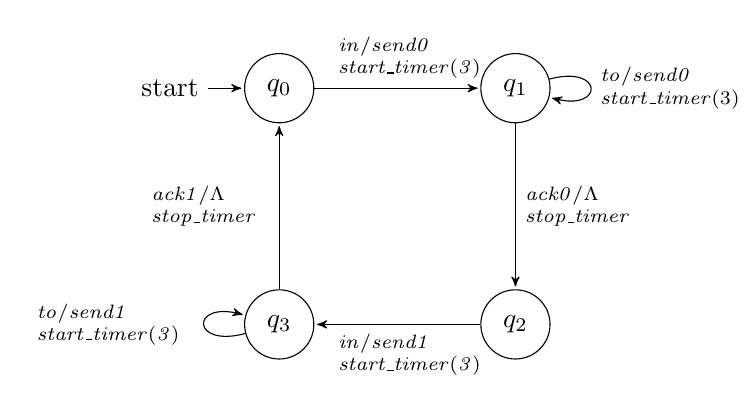
\begin{tikzpicture}[->,>=stealth',shorten >=1pt,auto,node distance=3cm,main node/.style={circle,draw,font=\sffamily\large\bfseries}]
  \node[initial, state] (1) {$q_0$};
  \node[state] (2) [right of=1] {$q_1$};
  \node[state] (3) [below of=2] {$q_2$};
  \node[state] (4) [below of=1] {$q_3$};

  \path[every node/.style={font=\sffamily\scriptsize}]
    (1) edge [text width=1.5cm] node {$\mathit{in}/\mathit{send0}$ \\ $\mathit{start\_timer(3)}$} (2)
    (2) edge [text width=1.5cm] node {$\mathit{ack0}/\Lambda$ \\ $\mathit{stop\_timer}$} (3)
        edge [loop right, text width=1.5cm] node {$\mathit{to}/\mathit{send0}$\\ $\mathit{start\_timer}(3)$ } (2)
    (3) edge [text width=1.5cm] node {$\mathit{in}/\mathit{send1}$ \\ $\mathit{start\_timer(3)}$} (4)
    (4) edge [text width=1.5cm] node {$\mathit{ack1}/\Lambda$ \\ $\mathit{stop\_timer}$} (1)
        edge [loop left, text width=2cm] node {$\mathit{to}/\mathit{send1}$\\ $\mathit{start\_timer(3)}$} (4);
\end{tikzpicture}
\caption{MM1T model of alternating-bit protocol sender}
\label{fig:abp}
\end{figure}
In the diagram we write $\mathit{start\_timer(n)}$ on a transition if this transition starts the
timer with value $n \in\nat^{>0}$, and we write $\mathit{stop\_timer}$ if the transition stops the timer.
We omit trivial self-loops: if some state $q$ does not have an outgoing $i$-transition in the diagram
then implicitly there is a transition $q \xrightarrow{i/\Lambda} q$.

In the model, input $\mathit{in}$ corresponds to a request from the upper layer to transmit data.
Initially, upon receipt of such a request, the sender builds a packet from the data and a sequence number $0$,
sends the packet over the network (output $\mathit{send0}$), and starts the timer with timeout value $3$.
If the sender receives an acknowledgement with the right sequence number $0$ (input $\mathit{ack0}$) 
then it stops the timer and jumps to state $q_2$.
Acknowledgement with the incorrect sequence number (input $\mathit{ack1}$) are ignored.
If no $\mathit{ack0}$ input arrives within $3$ timeunits, a timeout occurs and the same packet is sent again.
The behavior in states $q_2$ and state $q_3$ is analogous to that in states $q_0$ and $q_1$, respectively,
with the roles of sequence numbers $0$ and $1$ swapped.
\end{example}

\paragraph{Semantics.}
We give two semantics for MM1Ts, an untimed and a timed one.

Functions $\delta$, $\lambda$ and $\tau$ are extended to sequences of inputs in the usual way.
We define, for all $q \in Q$, $i \in I$ and $\sigma \in I^{\ast}$:
\begin{eqnarray*}
\delta(q, \epsilon) = q & , & \delta (q, i \; \sigma) = \delta(\delta(q,i), \sigma),\\
\lambda(q, \epsilon) = \epsilon & ,& \lambda(q, i \;\sigma) = \lambda(q,i) \; \lambda(\delta(q,i),\sigma),\\
\tau(q, \epsilon) = \epsilon &, & \tau(q, i \;\sigma) = \tau(q,i) \; \tau(\delta(q,i),\sigma).
\end{eqnarray*}
The untimed semantics of a MM1T $\M$ is given by the function $U_{\M}$ that assigns to each input sequence $\sigma \in I^{\ast}$
the pair $U_{\M}(\sigma) = (\lambda(q_0, \sigma), \tau(q_0, \sigma))$.
MM1Ts $\M$ and $\N$ are \emph{untimed equivalent}, written $\M \approx_{\mathit{untimed}} \N$, iff $U_{\M} = U_{\N}$.
%
Let $\sigma = i_1 \cdots i_k \in I^{\ast}$,
$\lambda(q_0, \sigma) = o_1 \cdots o_k$, and
$\tau(q_0, \sigma) = n_1 \cdots n_k$.
Then we say the sequence $i_1 o_1 n_1 i_2 o_2 n_2 \cdots i_k o_k n_k$ is a \emph{trace} of $\M$.
It is easy to see that $\M$ and $\N$ are untimed equivalent iff they have the same traces.

The timed semantics, which is slightly more involved, describes the real-time behavior of a MM1RT.
This semantics is defined by associating an infinite state transition system to a MM1T that describes all possible
configurations and transitions between them.
A \emph{configuration} of a MM1T is a pair $(q,t)$, where $q \in Q$ is a state and $t \in \bbbr^{\geq 0} \cup \{\infty\}$ 
specifies the value of the timer. We refer to the pair $(q_0, \infty)$ as the \emph{initial configuration}.
If $t = \infty$ then we say that the timer has been \emph{stopped}, otherwise it is \emph{running}.
Using four rules we define a transition relation that describes how one configuration may evolve into another.
For all $q, q' \in Q$, $i \in I$, $o \in O$, $t \in \bbbr^{\geq 0} \cup \{\infty\}$, $d \in \bbbr^{>0}$, and
$n \in \nat^{>0} \cup \{ \infty \}$,
\[
\frac{d \leq t}{(q,t) \xrightarrow{d} (q,t-d)} \hspace{1em}
\frac{q \xrightarrow{\mathit{to}/o,n} q'}{(q,0) \xrightarrow{\mathit{to}/o} (q',n)} \hspace{1em}
\frac{i \neq \mathit{to} ,~  q \xrightarrow{i/o,n} q'}{(q,t) \xrightarrow{i/o} (q',n)} \hspace{1em}
\frac{q\xrightarrow{i/o} q'}{(q,t) \xrightarrow{i/o} (q',t)}
\]
The first rule states that the value of the timer decreases when time advances, and
time can advance as long as the value of the timer is nonzero.
Here we use the convention that $\infty - d = \infty$, for any $d \in \bbbr$. This implies that when the
timer has been stopped time may advance indefinitely.
The second rule says that a timeout event occurs as soon as the timer has reached value $0$.
The third rule describes the transitions in response to a regular input, which may either start or stop the timer,
and the fourth rule describe transitions in which the timer is not affected.
A \emph{timed word} over inputs $I$ and outputs $O$ is a sequence $w = (i_0, o_0, t_0), (i_1, o_1, t_1) \cdots (i_k, o_k, t_k)$, where each $i_j \in I$, each $o_j \in O$, and each $t_j \in \bbbr^{\geq 0}$.
For a timed word $w = (i_0, o_0, t_0), (i_1, o_1, t_1) \cdots (i_k, o_k, t_k)$, a \emph{run} of MM1T $\M$ over $w$ is
a sequence 
\begin{eqnarray*}
\alpha & = & C_0 \xrightarrow{t_0} C'_0 \xrightarrow{i_0/o_0} C_1 \xrightarrow{t_1} C'_1 \xrightarrow{i_1/o_1} C_2 \cdots
\xrightarrow{t_k} C'_k \xrightarrow{i_k/o_k} C_{k+1}
\end{eqnarray*}
of transitions of $\M$ such that each $C_j, C'_j$ is a configuration of $\M$ and $C_0$ is the initial configuration.
Note that, since MM1Ts are deterministic, for each timed word $w$ there exists at most one run over $w$.
We say $w$ is a timed word of $\M$ if there exists a run of $\M$ over $w$.
Two MM1Ts $\M$ and $\N$ with the same sets of inputs are \emph{timed equivalent}, denoted $\M \approx_{\mathit{timed}} \N$, iff 
they have the same sets of observations.

\paragraph{Note}
The timed semantics is an idealization of the behavior of a real SUT: in a real system an input/output
interaction will always take a bit of time and will thus not be instantaneous.
This issue will be discussed in more detail in Section XX.
Note that a MM1T can be viewed as a very restricted type of timed automaton.

Although the definitions are quite different, it turns out that timed and untimed equivalence are almost the same.

\begin{theorem}
\label{untimedimpliestimed}
$\M \approx_{\mathit{untimed}} \N$
implies
$\M \approx_{\mathit{timed}} \N$.
\end{theorem}
\begin{proof}
Assume $\M \approx_{\mathit{untimed}} \N$ and assume
$w = (i_0, o_0, t_0), (i_1, o_1, t_1) \cdots (i_k, o_k, t_k)$ is an observation of $\M$.
Since $\approx_{\mathit{untimed}}$ is symmetric, it suffices to prove that $w$ is an observation of $\N$.

Because $w$ is an observation of $\M$, $\M$ has a run over $w$:
\[
C_0 \xrightarrow{t_0} C'_0 \xrightarrow{i_0/o_0} C_1 \xrightarrow{t_1} C'_1 \xrightarrow{i_1/o_1} C_2 \cdots
\xrightarrow{t_k} C'_k \xrightarrow{i_k/o_k} C_{k+1}
\]
Let $C_j = (q_j, u_i)$ and $C'_j = (q_j, u'_j)$, for all $j$.
Then $\M$ has a corresponding sequence of transitions:
\[
q_0 \xrightarrow{i_0/o_0, n_0} q_1 \xrightarrow{i_1/o_1, n_1} \cdots \xrightarrow{i_k/o_k, n_k} q_{k+1} .
\]
Let $\sigma = i_0 \cdots i_k$. Since $\M \approx_{\mathit{untimed}} \N$, $U_\M (\sigma) = U_\N (\sigma)$.
Therefore, $\N$ has a sequence of transitions:
\[
r_0 \xrightarrow{i_0/o_0, n_0} r_1 \xrightarrow{i_1/o_1, n_1} \cdots \xrightarrow{i_k/o_k, n_k} r_{k+1} .
\]
with all $r_j$ states of $\N$ and $r_0$ the initial state of $\N$. 
Let $D_j = (r_j, u_i)$ and $D'_j = (r_j, u'_j)$, for all $j$.
Then it is routine to check that
\[
D_0 \xrightarrow{t_0} D'_0 \xrightarrow{i_0/o_0} D_1 \xrightarrow{t_1} D'_1 \xrightarrow{i_1/o_1} D_2 \cdots
\xrightarrow{t_k} D'_k \xrightarrow{i_k/o_k} D_{k+1}
\]
is a run over $w$ of $\N$.
Thus $w$ is an observation of $\N$, as required.
\end{proof}

The converse of the implication of Theorem~\ref{untimedimpliestimed} does not hold, due to two technical problems.
The first problem is that in the timed semantics there can never be a timeout
in configurations where the timer is stopped, whereas in the untimed semantics a timeout is possible in every state.
The second problem is that in configurations where the timer is stopped, there is no observable difference between transitions that stop the timer and transitions that do not affect the timer.
In order to deal with these problems, we introduce the subclass of well-formed MM1Ts.
We show that
(a) for every MM1T there is a well-formed MM1T that is timed equivalent to it, and
(b) on well-formed MM1Ts the timed and the untimed semantics agree.

A MM1T is \emph{well-formed} if there exists a function $\mathit{timer}: Q \rightarrow \{ \mathit{on}, \mathit{off} \}$
such that:
\begin{enumerate}
\item
$\mathit{timer}(q_0) =  \mathit{off}$,
\item
if $q \xrightarrow{i/o, n} q'$ and $n \in \nat^{>0}$ then $\mathit{timer}(q') = \mathit{on}$,
\item
if $\mathit{timer}(q) =  \mathit{off}$ then $q \xrightarrow{\mathit{to}, \Lambda} q$,
\item
if $q \xrightarrow{i/o, \infty} q'$ then $\mathit{timer}(q) = \mathit{on}$ and $\mathit{timer}(q') = \mathit{off}$, and
\item
if $q \xrightarrow{i/o} q'$ then $\mathit{timer}(q)= \mathit{timer}(q')$.
\end{enumerate}

\begin{theorem}
For every MM1T $\M$ there exists a well-formed MM1T $\N$ with at most twice as many states such that 
$\M \approx_{\mathit{timed}} \N$.
\end{theorem}
\begin{proof}
Let $\M = (I, O, Q, q_0, \delta, \lambda, \tau)$ be a MM1T. 
We construct a well-formed MM1T $\N= (I, O, Q', q'_0, \delta', \lambda', \tau')$ that is timed equivalent to $\M$ 
by adding an extra bit to the state that records whether the timer is switched on or off.
We define $Q' = Q \times \{ \mathit{true}, \mathit{false} \}$ and $q'_0 = (q_0, \mathit{false})$.
Functions $\delta'$, $\lambda'$ and $\tau'$ are defined by the following five rules,
for all $q, q' \in Q$, $i \in I$, $o \in O$, $n \in \nat^{>0}$, and $b \in \{ \mathit{true}, \mathit{false} \}$,
\[
\frac{q \xrightarrow{i/o, n} q' ,~ i = \mathit{to} \Rightarrow b = \mathit{true}}
{(q,b) \xrightarrow{i/o, n} (q', \mathit{true})} \hspace{2em}
(q, \mathit{false}) \xrightarrow {\mathit{to}, \Lambda} (q, \mathit{false})
\]
\[
\frac{q \xrightarrow{i/o, \infty} q'}{(q, \mathit{true}) \xrightarrow{i/o, \infty} (q', \mathit{false})} \hspace{1em}
\frac{q \xrightarrow{i/o, \infty} q'}{(q, \mathit{false}) \xrightarrow{i/o} (q', \mathit{false})} \hspace{1 em}
\frac{q \xrightarrow{i/o} q'}{(q, b) \xrightarrow{i/o} (q', b)}
\]
The behavior of $\M$ and $\N$ is the same,
except that all $\mathit{to}$-transitions from states where the timer is off are replaced by trivial self loops (second rule),
and all transitions that stop the timer when it is already off are replaced by transitions that do not affect the timer (fourth rule).
It is straightforward to check that MM1T $\N$ is well-formed (by using
the $\mathit{timer}$ function that projects each state $(q, b)$ to its second component $b$)
and has twice as many states as $\M$.

In order to show that $\M \approx_{\mathit{timed}} \N$, we define a bisimulation relation between $\M$ and $\N$.
Let $R$ be the relation between configurations of $\M$ and $\N$ defined by:
\begin{eqnarray*}
R & = & \{ ((q,t), ((q, \mathit{true}), t)) \mid q \in Q,~ t \in \bbbr^{\geq 0} \} \cup\\
& & \{ ((q,\infty), ((q, \mathit{false}), \infty)) \mid q \in Q \}.
\end{eqnarray*}
Via a routine case distinction one can check that $R$ is a (strong) bisimulation relation between the infinite 
state transition systems associated to $\M$ and $\N$.
Clearly, strong bisimularity of transition systems implies equility of their sets of observations.
\end{proof}

Suppose that $\M = (I, O, Q, q_0, \delta, \lambda, \tau)$ is a well-formed MM1T and suppose that
$\beta = i_0 o_0 n_0 i_1 o_1 n_1 \cdots i_k o_k n_k$ is a trace of $\M$.
Then, by inspection of trace $\beta$, we can figure out whether the timer is on or off
after input sequence $\sigma = i_0 \cdots i_k$.
Define the value $\mathit{timer}(\beta) \in \{ \mathit{true}, \mathit{false} \}$ recursively as follows:
If $k=0$ then $\mathit{timer}(\beta) = \mathit{false}$. If $k > 0$ then
\begin{eqnarray*}
\mathit{timer}(\beta) & = & \left\{ \begin{array}{ll} 
\mathit{true} & \mbox{if } n_k \in\nat\\
\mathit{false} & \mbox{if } n_k = \infty\\
\mathit{timer}(\beta') & \mbox{if } n_k = \perp
\end{array}\right.
\end{eqnarray*}
with $\beta' = i_1 o_1 n_1 i_2 o_2 n_2 \cdots i_{k-1} o_{k-1} n_{k-1}$.
%
The following lemma is easy to prove by induction on the length of $\beta$:
\begin{lemma}
\label{timer lemma}
$\mathit{timer}(\beta) = \mathit{timer}(\delta(q_0, \sigma))$.
\end{lemma}

We call trace $\beta$ \emph{realizable} if no timeouts occur when the timer is off, that is,
for all $l < k$,
\begin{eqnarray*}
i_{l+1} = \mathit{to} & \Rightarrow & \mathit{timer} (i_1 o_1 n_1 i_2 o_2 n_2 \cdots i_l o_l n_l) = \mathit{true}
\end{eqnarray*}

For each realizable trace $\beta$ we may construct a corresponding run (thence the qualification ``realizable'')
\begin{eqnarray*}
\alpha & = & C_0 \xrightarrow{t_0} C'_0 \xrightarrow{i_0/o_0} C_1 \xrightarrow{t_1} C'_1 \xrightarrow{i_1/o_1} C_2 \cdots
\xrightarrow{t_k} C'_k \xrightarrow{i_k/o_k} C_{k+1}
\end{eqnarray*}
We call run $\alpha$ \emph{eager} if each transition is taken as soon as it is enabled, that is,
$i_j \neq \mathit{to} \Rightarrow t_j = 0$.
Then, in fact, for each realizable trace $\beta$ there is a unique eager run that corresponds to it.
If $\alpha$ is eager then the value $u_j$ of the timer in configuration $C_j$ is given by $u_0 = \infty$ and, for $j>0$,
\begin{eqnarray*}
u_j & = & \left\{ \begin{array}{ll} 
n_{j-1} & \mbox{if } n_{j-1} \in \nat^{>0} \cup \{\infty\}\\
u_{j-1} & \mbox{otherwise}
\end{array} \right.
\end{eqnarray*}
If $\alpha$ is eager then the timed word $w$ that corresponds to it is the sequence
$w = (i_0, o_0, t_0), (i_1, o_1, t_1) \cdots (i_k, o_k, t_k)$,
where, for all $j$,
\begin{eqnarray*}
t_j & = & \left\{ \begin{array}{ll} 
u_j & \mbox{if } i_j = \mathit{to}\\
0   & \mbox{otherwise}
\end{array}\right.
\end{eqnarray*}
Note that trace $\beta$ contains all the information required to compute $w$.

If $\beta$ is a trace of a well-formed MM1T and we insert a triple ``$\mathit{to} \; \Lambda\; \perp$'' at a point where 
the timer is off, then the result will again be a trace of the MM1T.
In fact, any trace from a MM1T can be obtained from a realizable trace by repeating this operation a number of times.
This implies the following lemma:

\begin{lemma}
\label{realizable}
Let $\M$ and $\N$ be well-formed MM1Ts with the same realizable traces.
Then  $\M \approx_{\mathit{untimed}} \N$.
\end{lemma}

\begin{theorem}
Let $\M$ and $\N$ be well-formed MM1Ts.
Then  $\M \approx_{\mathit{timed}} \N$ implies $\M \approx_{\mathit{untimed}} \N$.
\end{theorem}
\begin{proof}
Suppose $\M \approx_{\mathit{timed}} \N$. 

By Lemma~\ref{realizable}, it suffices to prove that $\M$ and $\N$ have the same realizable traces.
Let $\beta$ be a realizable trace of $\M$.
We prove by induction on the length of $\beta$ that $\beta$ is a realizable trace of $\N$ (the other inclusion follows by symmetry).

The base case is trivial, since the empty trace is a realizable trace of $\N$.

Now suppose the length of $\beta$ is $3(k+1)$, for some $k$.
Let $\beta = \gamma \; i \; o \; n$.
Then $\gamma$ is the prefix of $\beta$ of length $3 k$.
Since $\gamma$ is a realizable trace of $\M$, by induction hypothesis, $\gamma$ is a realizable trace of $\N$.
Let $\alpha$ and $\alpha'$ be the unique eager runs that correspond to $\gamma$ in $\M$ and $\N$, respectively.
Then both $\alpha$ and $\alpha'$ have the same timed word $w$. 
Let $q$ and $q'$ be the final states of $\alpha$ and $\alpha'$, respectively.
By Lemma~\ref{timer lemma}, either the timer is on both in $q$ and $q'$, or the timer is off in both $q$ and $q'$.
Moreover, in the final configurations of both runs the timers have the same value $t$.

If the last input $i$ from trace $\beta$ is different from $\mathit{to}$, then
$w \; (i \; o \; 0)$ is a timed word of $\M$.
Since $\M \approx_{\mathit{timed}} \N$, $w \; (i \; o \; 0)$ is also a timed word of $\N$.
Hence $\N$ has a realizable trace $\beta' \; i \; o \; n'$, and it remains to show $n = n'$.
We consider three cases:
\begin{enumerate}
\item
If $n = \infty$, then $\M$ has timed words $w \; (i \; o \; 0) \; (i \; o' \; d)$, for some output $o'$ and for any $d \in\bbbr^{\geq 0}$.
By well-formedness, the timer is on in state $q$, and thus it is also on in state $q'$.
Since $\N$ has the same timed words as $\M$, and since the timer is off in $q'$, we may conclude $n' = \infty$.
\item
If the timer is off in $q$ and $n = \perp$, then $\M$ has timed words $w \; (i \; o \; 0) \; (i \; o' \; d)$, for some output $o'$ and for any $d \in\bbbr^{\geq 0}$.
Since $\N$ has the same timed words as $\M$, since the timer is off in $q'$, 
and since $\N$ is well-formed, we may conclude $n' = \perp$.
\item 
If the timer is on in $q$ and $n = \perp$, then $\M$ has a timed word $w \; (i \; o \; \frac{1}{2}) \; (\mathit{to} \; o' \; t- \frac{1}{2})$, for some output $o'$.
Since $\N$ has the same timed words as $\M$, and since the value of the timer in state $q'$ is $t$, we may conclude $n' = \perp$.
\item
If $n \in \nat^{\geq 0}$, then $\M$ has a timed word $w \; (i \; o \; \frac{1}{2}) \; (\mathit{to} \; o' \; n)$, for some output $o'$.
Since $\N$ has the same timed words as $\M$, and since the value of the timer in state $q'$ is $t$, we may conclude $n' = n$.
\end{enumerate}
If the last input $i$ from trace $\beta$ equals $\mathit{to}$, then
$w \; (\mathit{to} \; o \; t)$ is a timed word of $\M$.
Since $\M \approx_{\mathit{timed}} \N$, $w \; (\mathit{to} \; o \; t)$ is also a timed word of $\N$.
Hence $\N$ has a realizable trace $\beta' \; \mathit{to} \; o \; n'$, and it remains to show $n = n'$.
By Definition~\ref{MM1T}, a timeout event either starts or stops the timer, and thus it suffices to consider the
following two cases:
\begin{enumerate}
\item
If $n = \infty$, then $\M$ has timed words $w \; (i \; o \; 0) \; (i \; o' \; d)$, for some output $o'$ and for any $d \in\bbbr^{\geq 0}$.
By well-formedness, the timer is on in state $q$, and thus it is also on in state $q'$.
Since $\N$ has the same timed words as $\M$, and since the timer is off in $q'$, we may conclude $n' = \infty$.
\end{enumerate}
\end{proof}

\newcommand{\natplus}{\nat^{>0}}
\newcommand{\realsplus}{\bbbr^{\geq 0}}
\newcommand{\delays}{\bbbr^{> 0}}
\newcommand{\stoptimer}{\mathit{kill}}
\newcommand{\tosymbol}{\mathit{to}}
\newcommand{\toevent}[1]{\mathit{to}[#1]}
\newcommand{\toevents}{\mbox{\sl TO}}
\newcommand{\extinputs}{\hat{I}}
\newcommand{\acttimers}{\mathit{active}}
\newcommand{\Head}[1]{\mathsf{Head}({#1})}
\newcommand{\Tail}[1]{\mathsf{Tail}({#1})}
\newcommand{\Last}[1]{\mathsf{Last}({#1})}
\newcommand{\expirable}{\mathit{expirable}}
\newcommand{\tvals}{\kappa}
\newcommand{\Vals}[1]{\mathit{Val}({#1})}
\newcommand{\delay}[2]{t_{[#1:#2]}}
\newcommand{\timerof}[2]{x_{#1}^{#2}}
\newcommand{\constrof}[1]{\phi_{#1}}
\newcommand{\Post}{\mathsf{Post}}
\newcommand{\beh}{\mathit{beh}}
\newcommand{\untime}{\mathit{untime}}
\newcommand{\run}{\mathit{pullback}}
\newcommand{\timedword}{\mathit{tw}}

\newcommand{\conc}{\cdot}
\newcommand{\tuple}[1]{\langle #1\rangle}
\newcommand{\set}[1]{\lbrace #1\rbrace}
\newcommand{\vect}[2]{{#1}_1 , \ldots , {#1}_{#2}}
\newcommand{\setcomp}[2]{\set{#1 ~:~ #2}}
\newcommand{\domof}[1]{\dom(#1)}
\newcommand{\ranof}[1]{\ran(#1)}
\newcommand{\vars}{\mathcal{X}}
\newcommand{\varsof}[1]{\vars(#1)}
\newcommand{\ctimers}{X}
\newcommand{\remap}{\pi}
\newcommand{\remapinst}{\rho}
\newcommand{\normalize}{\gamma}
\newcommand{\normalizeof}[2]{\normalize_{#2}^{#1}}
\newcommand{\timerbij}{\gamma}
\newcommand{\timerequiv}{\pi}
\newcommand{\extendedby}{\lhd}
\newcommand{\uttrace}{\textsf{tr}}
\newcommand{\uttraceof}[1]{\uttrace(#1)}
\newcommand{\uttracesof}[1]{\textsf{Tr}(#1)}
\newcommand{\strace}{\textsf{tr}_s}
\newcommand{\ssuffix}{v_s}
\newcommand{\suftraces}{\textsf{Tr}_s}
\newcommand{\pinpof}[1]{\textit{inp}_p(#1)}
\newcommand{\sinpof}[1]{\textit{inp}_s(#1)}
\newcommand{\symbinpof}[1]{\textit{symbinp}(#1)}
\newcommand{\word}{w}
\newcommand{\smap}{{\cal O}}
\newcommand{\smappre}{{\cal O_p}}
\newcommand{\smapsuf}{{\cal O_s}}
\newcommand{\obspre}{{\cal O_U}}

\section{MMTs}

\begin{example}
%As a first running example, 
The MM1T of Figure~\ref{fig:abp} presents a simplified model of the sender from 
the alternating-bit protocol, adapted from \cite[Figure 3.15]{KR13}.
\begin{figure}[h]
\centering
\vspace{-2 em}
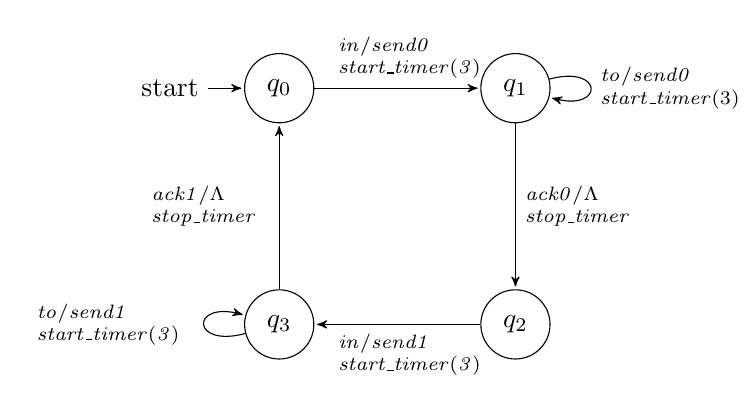
\begin{tikzpicture}[->,>=stealth',shorten >=1pt,auto,node distance=3cm,main node/.style={circle,draw,font=\sffamily\large\bfseries}]
  \node[initial, state] (1) {$q_0$};
  \node[state] (2) [right of=1] {$q_1$};
  \node[state] (3) [below of=2] {$q_2$};
  \node[state] (4) [below of=1] {$q_3$};

  \path[every node/.style={font=\sffamily\scriptsize}]
    (1) edge [text width=1.5cm] node {$\mathit{in}/\mathit{send0}$ \\ $\mathit{start\_timer(3)}$} (2)
    (2) edge [text width=1.5cm] node {$\mathit{ack0}/\Lambda$ \\ $\mathit{stop\_timer}$} (3)
        edge [loop right, text width=1.5cm] node {$\mathit{to}/\mathit{send0}$\\ $\mathit{start\_timer}(3)$ } (2)
    (3) edge [text width=1.5cm] node {$\mathit{in}/\mathit{send1}$ \\ $\mathit{start\_timer(3)}$} (4)
    (4) edge [text width=1.5cm] node {$\mathit{ack1}/\Lambda$ \\ $\mathit{stop\_timer}$} (1)
        edge [loop left, text width=2cm] node {$\mathit{to}/\mathit{send1}$\\ $\mathit{start\_timer(3)}$} (4);
\end{tikzpicture}
\caption{MM1T model of alternating-bit protocol sender}
\label{fig:abp}
\end{figure}
In the diagram we write $\mathit{start\_timer(n)}$ on a transition if this transition starts the
timer with value $n \in\nat^{>0}$, and we write $\mathit{stop\_timer}$ if the transition stops the timer.
We omit trivial self-loops: if some state $q$ does not have an outgoing $i$-transition in the diagram
then implicitly there is a transition $q \xrightarrow{i/\Lambda} q$.

In the model, input $\mathit{in}$ corresponds to a request from the upper layer to transmit data.
Initially, upon receipt of such a request, the sender builds a packet from the data and a sequence number $0$,
sends the packet over the network (output $\mathit{send0}$), and starts the timer with timeout value $3$.
If the sender receives an acknowledgement with the right sequence number $0$ (input $\mathit{ack0}$) 
then it stops the timer and jumps to state $q_2$.
Acknowledgement with the incorrect sequence number (input $\mathit{ack1}$) are ignored.
If no $\mathit{ack0}$ input arrives within $3$ timeunits, a timeout occurs and the same packet is sent again.
The behavior in states $q_2$ and state $q_3$ is analogous to that in states $q_0$ and $q_1$, respectively,
with the roles of sequence numbers $0$ and $1$ swapped.
\end{example}

\subsection{MMTs}
We assume an unbounded set $X$ of {\em timers};
we use $x$, $x_1$, $x_2$, etc.\ to range over timers.
Let $\toevents$ be the set of {\em timeout events} of form
$\toevent{x}$ for $x \in X$.
For a set $I$, let $\extinputs$ be $I \cup \toevents$.

We write $A \hookrightarrow B$ for the set of partial functions from $A$ to $B$.
With $f \lceil A$ we denote the restriction of function $f$ to $\domof{f} \cap A$.
For arbitrary functions $f$ and $g$, $f [g]$ is the function with domain $\domof{f}$ that behaves like $f$
on $\domof{f} \setminus \domof{g}$ and like $g$ on $\domof{f} \cap \domof{g}$.

\begin{definition}
\label{def:MMT}
A \emph{Mealy machine with timers (MMT)} is a tuple
\\
$\M = (I, O, Q, q_0, \vars, \delta, \lambda, \remap)$, where
\begin{itemize}
\item
$I$ is a finite set of input events,
\item
$O$ is a finite set of outputs, containing a special default output $\Lambda$,
\item
$Q$ is a finite set of states,
\item
$q_0 \in Q$ is the initial state,
\item
$\vars$ maps each state $q \in Q$ to a finite set of timers $\varsof{q}$, with $\varsof{q_0} = \emptyset$,
\item
$\delta: Q \times \extinputs \hookrightarrow  Q$ is a transition function,
%with $\delta(q,i)$ defined iff $q \in Q$ and $i \in I \cup \{ \toevent{x} \mid x \in \varsof{q} \}$, 
\item
$\lambda: Q \times \extinputs \hookrightarrow O$ is an output function, 
\item
$\remap : Q \times \extinputs \hookrightarrow (X \hookrightarrow \natplus)$ is a timer initialization function.
Let $q \in Q$, $i \in \extinputs$, $q'=\delta(q,i)$ and $\rho=\remap(q,i)$. 
We require that $\varsof{q'} \setminus \varsof{q} \subseteq \domof{\rho} \subseteq\varsof{q'}$. Moreover
  if $i=\toevent{x}$, for some $x$, then $x \not\in \varsof{q'} \setminus \domof{\rho}$.
\end{itemize}
We require that input events are always enabled and timeout events are only enabled
for timers that are active in the current state:
\marginpar{Explain injectivity is required for determinism}
for $q \in Q$ and $i \in \extinputs$,  $\delta(q,i)$, $\lambda(q,i)$ and $\pi(q,i)$ are defined iff either
$i \in I$ or $i=\toevent{x}$, for some $x \in\varsof{q}$.
We write $q \xrightarrow{i/o,\rho} q'$ if $\delta(q,i) = q'$, $\lambda(q,i)= o$ and $\remap(q,i) = \rho$.
\end{definition}
The restart function $\remap$ determines how timers are affected when an event $i$ occurs in state $q$.
Basically, there are four things that may happen.
\marginpar{Add Venn diagram to illustrate situation.}
Let $q \in Q$, $i \in \extinputs$, $\delta(q,i)=q'$ and $\remap(q,i)=\rho$.
\begin{enumerate}
\item
If $x \in\varsof{q} \setminus \varsof{q'}$ then input $i$ \emph{stops} timer $x$.
\item
If $x \in \varsof{q'} \setminus \varsof{q}$ then $i$ \emph{starts} timer $x$ with value $\rho(x)$.
\item
If $x \in \varsof{q} \cap \domof{\rho}$ then $i$ \emph{restarts} timer $x$ with value $\rho(x)$.
\item
Finally, if $x \in \varsof{q'} \setminus \domof{\rho}$ then timer $x$ is \emph{unaffected} by $i$.
\end{enumerate}
Hence, when timer $x$ expires (i.e., event $\toevent{x}$ occurs) it is either stopped or restarted.

\paragraph{Semantics.}
The semantics of MMT $\M = (I, O, Q, q_0, \vars, \delta, \lambda, \remap)$ is defined via an infinite state transition system that describes all possible
configurations and transitions between them.
A \emph{valuation} is a partial function
$\tvals : X \hookrightarrow \realsplus$, defined on a finite subset of $X$, that assigns nonnegative real numbers as values to timers.
We write $\Vals{Y}$ for the set of valuations with domain $Y \subseteq X$.
A \emph{configuration} of an MMT is a pair $(q,\tvals)$, where $q \in Q$ is a state and $\tvals\in\Vals{\varsof{q}}$ is a valuation.
The \emph{initial configuration} is the pair $(q_0, \tvals_0)$, where $\tvals_0$ is the empty function.
Valuations and configurations can be modified by the occurrence of discrete events (inputs or timeouts) and by
the occurrence of delays.
If $\tvals$ is a valuation in which all timers
have a value of at least $d$, then $d$ units of time may pass. As a result this delay the value of all the timers is decremented by $d$.
Formally, for $\tvals, \tvals'$ valuations and delay $d \in \delays$, we define a delay transition predicate by
\marginpar{The whole robustness analysis becomes easy/trivial if we assume $d>0$, because then 
a time delay precedes each input, allowing us to fidget with the timing of this input. Argument against this change is that
in a concurrent setting we may not exclude simulaneous inputs.}
\begin{eqnarray*}
\tvals \xrightarrow{d} \tvals' & \Leftrightarrow & [\domof{\tvals} = \domof{\tvals'} \wedge \forall x \in\domof{\tvals} : \tvals'(x) = \tvals(x) - d ].
\end{eqnarray*}
If the current valuation is $\tvals$, then a timeout event $\toevent{x}$ may occur only if $\tvals(x)=0$.
If an input or a timeout event occurs, a valuation is updated as specified by timer initialization function $\rho$.
The values of timers that are not affected by $\rho$ remain unchanged.
Formally, for $\tvals, \tvals'$ valuations, $i \in \extinputs$, $o \in O$ and $\rho \in X \hookrightarrow \natplus$,
we define a discrete transition predicate by
\begin{eqnarray*}
\tvals \xrightarrow{i/o, \rho}  \tvals' & \Leftrightarrow & [ \domof{\tvals'} \setminus \domof{\tvals}  \subseteq \domof{\rho} \subseteq \domof{\tvals'} ~ \wedge\\
&& \tvals' =  \tvals'[\tvals][\rho] ~ \wedge \\
&& \forall x \in X : i=\toevent{x} \Rightarrow (\tvals(x) = 0 \wedge x \not\in\domof{\tvals'} \setminus \domof{\rho})].
\end{eqnarray*}
Transition predicates $\xrightarrow{d}$ and $\xrightarrow{i/o, \rho}$ can be easily lifted to configurations.
For all configurations $(q, \tvals)$, $(q', \tvals')$ of an MMT $\M$,
\[
\frac{q = q' \quad \tvals \xrightarrow{d} \tvals'}{(q,\tvals) \xrightarrow{d} (q',\tvals')}
\quad\quad
  \frac{q \xrightarrow{i/o,\remapinst} q' \quad \tvals \xrightarrow{i/o, \rho} \tvals'}{(q,\tvals) \xrightarrow{i/o} (q',\tvals')}
\]
A \emph{timed run} of $\M$ over $w$ is a sequence 
\begin{eqnarray*}
\alpha & = & C_0 \xrightarrow{d_1} C'_0 \xrightarrow{i_1/o_1} C_1 \xrightarrow{d_2} C'_1 \xrightarrow{i_2/o_2} C_2 \cdots
\xrightarrow{d_k} C'_{k-1} \xrightarrow{i_k/o_k} C_{k}
\end{eqnarray*}
of transitions between configurations $C_j, C'_j$ of $\M$, where $C_0$ is the initial configuration.
%Note that, since MMTs are deterministic (if we allow to observe the
%identities of timers in timeout events),
%for each timed word $w$ there exists at most one run over $w$.
A \emph{timed word} over inputs $I$ and outputs $O$ is a sequence
\begin{eqnarray*}
w & = &  d_1 ~ i_1 ~ o_1 ~ d_2 ~ i_2 ~ o_2 \cdots d_k ~ i_k ~ o_k,
\end{eqnarray*}
where $d_j \in \delays$, $i_j \in I \cup \{ \mathit{to} \}$, and $o_j \in O$.
To each timed run $\alpha$ we can associate a \emph{timed word} by forgetting the configurations and the names of timers
in timeout events:
\begin{eqnarray*}
\timedword(\alpha) & = & d_1 ~ i'_1 ~ o_1 ~ d_2 ~ i'_2 ~ o_2 \cdots d_k ~ i'_k ~ o_k, \mbox{ where for all } j\\
i'_j & = & \left\{ \begin{array}{ll}
i_j & \mbox{if } i_j \in I\\
\mathit{to} & \mbox{if } i_j \in \toevents
\end{array} \right.
\end{eqnarray*}
The idea is that, that when we observe an output that is not directly triggered by an input, we may
may conclude that a timeout occurred. We cannot observe, however, which timer timed out.

We say $w$ is a timed word of $\M$ if $\M$ has a timed run $\alpha$ with $w = \timedword(\alpha)$.
%
Two MMTs $\M$ and $\N$ with the same sets of inputs are \emph{timed equivalent}, denoted $\M \approx_{\mathit{timed}} \N$, iff 
they have the same sets of timed words.

\paragraph{Remark.}
Note that we assume that in a timed run each discrete transition is preceded by a nonzero delay.
This assumption is a crucial requirement for the learning algorithm that we present in this paper.
The idea that multiple consecutive discrete transitions may occur in zero time is a useful abstraction in synchronous
programming and in the theory of timed automata, but unfortunately it appears to be incompatible with our approach.


\paragraph{Nondeterminism.}
Due to our assumption that we cannot observe the name of the timer in a timeout event, an MMT may exhibit nondeterministic
behavior: even if we offer exactly the same inputs at exactly the same time, different outputs may occur in different runs. 
The MMT of Figure~\ref{fig:nondeterminism}, for instance, accepts both the timed words
$1 ~ i ~ o ~ 1 ~ \mathit{to} ~ o'$ and $1 ~ i ~ o ~ 1 ~ \mathit{to} ~ o''$.
(For clarity, we omit some self-loop transitions in the state/transition diagram.)
\begin{figure}[ht]
\begin{center}
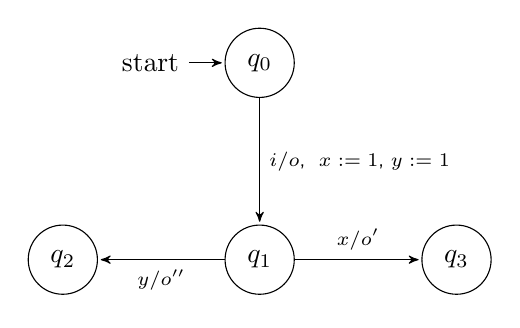
\begin{tikzpicture}[->,>=stealth',shorten >=1pt,auto,node distance=2.5cm,main node/.style={circle,draw,font=\sffamily\large\bfseries}]
  \node[initial, state] (1) {$q_0$};
  \node[state] (2) [below of=1] {$q_1$};
  \node[state] (3) [right of=2] {$q_3$};
  \node[state] (4) [left of=2] {$q_2$};

  \path[every node/.style={font=\sffamily\scriptsize}]
    (1) edge node {$i/o$, $~x:=1$, $y:=1$} (2)  
    (2) edge  node {$\toevent{x}/o'$} (3)
      edge  node {$\toevent{y}/o''$} (4);
\end{tikzpicture}
\caption{An MMT with nondeterministic behavior}
\label{fig:nondeterminism}
\end{center}
\end{figure}
In order to rule out this type of nondeterminism, it is not enough to require that the timer initializations are injective,
that is, it is not allowed to assign the same value to multiple timers in a single transition.
This is illustrated by the MMT of Figure~\ref{fig:nondeterminism2}, which accepts both the timed words
$1 ~ i ~ o ~ 1 ~ \mathit{to} ~ o'~ 1 ~ \mathit{to} ~ o'$ and $1 ~ i ~ o ~ 1 ~ \mathit{to} ~ o' ~ 1 ~ \mathit{to} ~ o''$.
\begin{figure}[ht]
\begin{center}
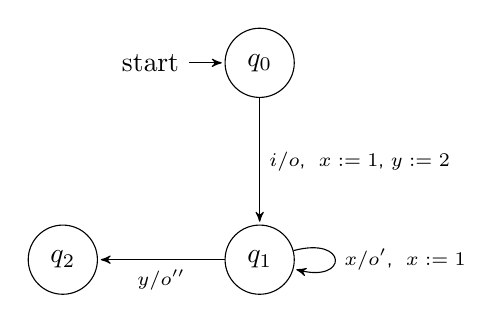
\begin{tikzpicture}[->,>=stealth',shorten >=1pt,auto,node distance=2.5cm,main node/.style={circle,draw,font=\sffamily\large\bfseries}]
  \node[initial, state] (1) {$q_0$};
  \node[state] (2) [below of=1] {$q_1$};
  \node[state] (4) [left of=2] {$q_2$};

  \path[every node/.style={font=\sffamily\scriptsize}]
    (1) edge node {$i/o$, $~x:=1$, $y:=2$} (2)  
    (2) edge  node {$\toevent{y}/o''$} (4)
      edge  [loop right] node {$\toevent{x}/o'$, $~x:=1$} (2);
\end{tikzpicture}
\caption{Another MMT with nondeterministic behavior}
\label{fig:nondeterminism2}
\end{center}
\end{figure}

The nondeterminism of the MMTs of Figures~\ref{fig:nondeterminism} and \ref{fig:nondeterminism2} is ``uncontrollable'' in the
sense that it occurs after any (nonempty) input sequence.
Figure~\ref{fig:nondeterminism3} gives an example of an MMT that exhibits nondeterminism when the second input occurs \emph{exactly} one timeunit after the first input: the MMT accepts behaviors
$7 ~ i ~ o ~ 1 ~ i ~ o ~ 1 ~ \mathit{to} ~ o'$ and $7 ~ i ~ o ~ 1 ~ i ~ o ~ 1 ~ \mathit{to} ~ o''$.
This type of nondeterminism is ``controllable'' in the sense that no nondeterminism will occur if we are careful
when selecting the timing of inputs.
\begin{figure}[ht]
\begin{center}
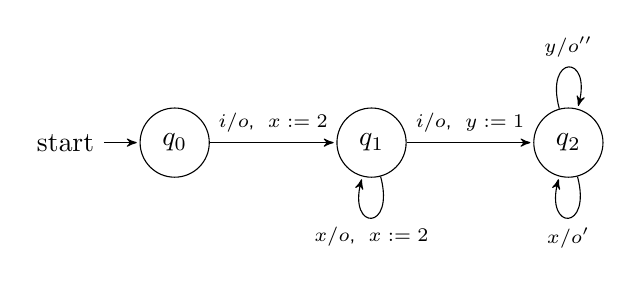
\begin{tikzpicture}[->,>=stealth',shorten >=1pt,auto,node distance=2.5cm,main node/.style={circle,draw,font=\sffamily\large\bfseries}]
  \node[initial, state] (1) {$q_0$};
  \node[state] (2) [right of=1] {$q_1$};
  \node[state] (3) [right of=2] {$q_2$};

  \path[every node/.style={font=\sffamily\scriptsize}]
    (1) edge node {$i/o$, $~x:=2$} (2)  
    (2) edge  node {$i/o$, $~y:=1$} (3)
      edge  [loop below] node {$\toevent{x}/o$, $~x:=2$} (2)
   (3) edge  [loop below] node {$\toevent{x}/o'$} (3)
   edge  [loop above] node {$\toevent{y}/o''$} (3);
\end{tikzpicture}
\caption{An MMT with ``controllable'' nondeterministic behavior}
\label{fig:nondeterminism3}
\end{center}
\end{figure}
Our learning algorithm applies to MMTs in which at most one timer is (re)started on each transition. Such MMTs do not
exhibit uncontrollable nondeterminism. The algorithm chooses the timing of the input events in such a way that no
nondeterministic behavior may arise.

\subsection{A product construction}
An \emph{untimed behavior} over inputs $I$, outputs $O$, and timers $Y \subseteq X$ is a sequence 
\begin{eqnarray*}
\beta & = & X_0 \xrightarrow{i_1/o_1, \rho_1} X_1  \xrightarrow{i_2/o_2, \rho_2} X_2 \cdots \xrightarrow{i_k/o_k, \rho_k} X_{k},
\end{eqnarray*}
where $X_0 \subseteq Y$ and, for each $j>0$,  $i_j \in \extinputs$, $o_j \in O$, $\rho_j \in X \hookrightarrow \natplus$, and
 $X_j \setminus X_{j-1}  \subseteq \domof{\rho_j} \subseteq X_j \subseteq Y$.
Moreover, if $i_j = \toevent{x}$, for some $j>0$, then $x \in X_{j-1}$ and $x \not\in X_j \setminus \domof{\rho_j}$.

An \emph{untimed run} of an MMT $\M$ is a sequence
\begin{eqnarray*}
\gamma & = & q_0 \xrightarrow{i_1/o_1, \rho_1} q_1  \xrightarrow{i_2/o_2, \rho_2} q_2 \cdots \xrightarrow{i_k/o_k, \rho_k} q_k
\end{eqnarray*}
of transitions of $\M$ that starts with the initial state $q_0$. 
To each untimed run $\gamma$ we can associate a corresponding untimed behavior by simply replacing all
states by their sets of timers:
\begin{eqnarray*}
\beh(\gamma) & = & \vars(q_0) \xrightarrow{i_1/o_1, \rho_1} \vars(q_1)  \xrightarrow{i_2/o_2, \rho_2} \vars(q_2) \cdots \xrightarrow{i_k/o_k, \rho_k} \vars(q_k).
\end{eqnarray*}
We say that $\beta$ is a untimed behavior of $\M$ if $\M$ has an untimed run $\gamma$ with $\beh(\gamma) = \beta$.
Note that the initial timer set of any untimed behavior of $\M$ is empty.

A \emph{timed behavior} over inputs $I$, outputs $O$, and timers $Y \subseteq X$ is an alternating sequence
\begin{eqnarray}
\label{timedbehavior}
\sigma & = & \tvals_0 \xrightarrow{d_1} \tvals'_0 \xrightarrow{i_1/o_1, \rho_1} \tvals_1 \xrightarrow{d_2} \tvals'_1 \xrightarrow{i_2/o_2, \rho_2} \tvals_2 \cdots
\xrightarrow{d_k} \tvals'_{k-1} \xrightarrow{i_k/o_k, \rho_k} \tvals_{k}
\end{eqnarray}
of delay predicates and event predicates with, for each $j$,
$\tvals_j, \tvals'_j$ valuations
with $\domof{\tvals_j} = \domof{\tvals'_j} \subseteq Y$ and,
for each $j>0$,  $d_j \in \delays$, $i_j \in \extinputs$, $o_j \in O$, and $\rho_j \in Y \hookrightarrow \natplus$.
To each timed behavior $\sigma$ we can associate a corresponding untimed behavior by forgetting the time
delays and by replacing valuations by their domain:
\begin{eqnarray*}
\untime(\sigma) & = & \domof{\tvals_0} \xrightarrow{i_1/o_1, \rho_1} \domof{\tvals_1}  \xrightarrow{i_2/o_2, \rho_2} \domof{\tvals_2} \cdots \xrightarrow{i_k/o_k, \rho_k} \domof{\tvals_k}.
\end{eqnarray*}
We say that untimed behavior $\beta$ is \emph{feasible} if there exists a timed behavior $\sigma$ such that $\untime(\sigma) = \beta$.
We can also associate a timed word to timed behavior $\sigma$ by forgetting the valuations and the initialization functions:
\begin{eqnarray*}
\timedword(\sigma) & = & d_ 1 ~ i_1 ~ o_1 ~ i_2 ~ o_2 \cdots d_k ~ i_k ~ o_k.
\end{eqnarray*} 
Let $\alpha$ be a timed run of an MMT $\M$: 
\begin{eqnarray*}
\alpha & = & (q_0, \tvals_0) \xrightarrow{d_1} (q_0, \tvals'_0) \xrightarrow{i_1/o_1} (q_1, \tvals_1) \xrightarrow{d_2} (q_1, \tvals'_1)  \cdots
 \xrightarrow{i_k/o_k} (q_k, \tvals_k).
\end{eqnarray*}
Then $\alpha$ can be projected both to an untimed run of $\M$
\begin{eqnarray*}
\untime (\alpha) & = & q_0 \xrightarrow{i_1/o_1, \rho_1} q_1  \xrightarrow{i_2/o_2, \rho_2} q_2 \cdots \xrightarrow{i_k/o_k, \rho_k} q_k
\end{eqnarray*}
(note that the $\rho_j$ are uniquely determined since $\M$ is deterministic) and to a timed behavior
\begin{eqnarray*}
\beh(\alpha) & = & \tvals_0 \xrightarrow{d_1} \tvals'_0 \xrightarrow{i_1/o_1, \rho_1} \tvals_1 \xrightarrow{d_2} \tvals'_1 \xrightarrow{i_2/o_2, \rho_2} \tvals_2 \cdots
\xrightarrow{d_k} \tvals'_{k-1} \xrightarrow{i_k/o_k, \rho_k} \tvals_{k}.
\end{eqnarray*}
Note that $\beh(\untime(\alpha))=\untime(\beh(\alpha))$ and $\timedword(\alpha) = \timedword(\beh(\alpha))$.
Thus the diagram of Figure~\ref{fig:diagram}, which summarizes the various types of runs and behaviors that we consider
in this article, commutes.
\begin{figure}[h]
\centering
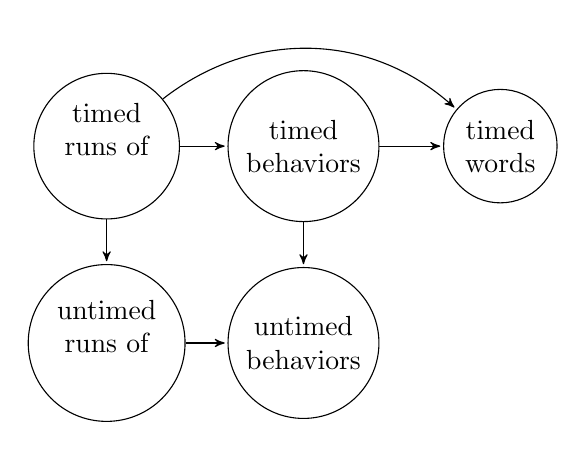
\begin{tikzpicture}[->,>=stealth',shorten >=1pt,auto,node distance=2.5cm,main node/.style={circle,draw,font=\sffamily\large\bfseries}]
  \node[state,align=center] (1) {timed \\ runs of\\ $\M$};
  \node[state,align=center] (2) [below of=1] {untimed \\ runs of\\ $\M$};
  \node[state,align=center] (3) [right of=1] {timed\\ behaviors};
  \node[state,align=center] (4) [right of=2] {untimed\\ behaviors};
  \node[state,align=center] (5) [right of=3] {timed \\words};

  \path[every node/.style={font=\sffamily\scriptsize}]
    (1) edge  node {$\untime$} (2)
        edge  node {$\beh$} (3)
        edge[bend left=40]  node {$\timedword$} (5)
    (2) edge  node {$\beh$} (4)
    (3) edge  node {$\untime$} (4)
        edge  node {$\timedword$} (5);
\end{tikzpicture}
\caption{Functions relating different types of runs and behaviors}
\label{fig:diagram}
\end{figure}
Conversely, if $\gamma$ is an untimed run  of $\M$ and $\sigma$ is a timed behavior such that $\beh(\gamma) = \untime(\sigma)$,
then there exists a unique timed run $\alpha$ of $\M$ with $\untime(\alpha) = \gamma$ and $\beh(\alpha) = \sigma$.
We refer to $\alpha$ as $\run(\gamma,\sigma)$.

\subsection{Untimed semantics}
We would, intuitively, like to let the untimed semantics of an MMT $\M$ be the set of its feasible untimed behaviors.
However, this semantics would then depend heavily on the names of the timers. Therefore, we define an equivalence relation
on untimed behaviors, which deems two untimed behaviors equivalent if there is a consistent renaming of timers that transforms
the one into the other.

Let $X_0,\ldots, X_k$ be a sequence of sets $X_j \subseteq X$ of timers.
An \emph{isomorphism} for $X_0,\ldots, X_k$ is a sequence $f = f_0 ,\ldots, f_k$ of bijections $f_j : X_j \rightarrow Y_j$ such that,
for all $j>0$, $f_j \lceil X_{j-1} = f_{j-1} \lceil X_j$ and $f_j (X_j \setminus X_{j-1}) \cap Y_{j-1} = \emptyset$.
If $f = f_0 ,\ldots, f_k$ is an isomorphism with $f_j : X_j \rightarrow Y_j$ and
\begin{eqnarray*}
\beta & = & X_0 \xrightarrow{i_1/o_1, \rho_1} X_1  \xrightarrow{i_2/o_2, \rho_2} X_2 \cdots \xrightarrow{i_k/o_k, \rho_k} X_{k}
\end{eqnarray*}
is an untimed behavior then $f(\beta)$ is the untimed behavior given by
\begin{eqnarray*}
f(\beta) & = & Y_0 \xrightarrow{i'_1/o_1, \rho'_1} Y_1  \xrightarrow{i'_2/o_2, \rho'_2} Y_2 \cdots \xrightarrow{i'_k/o_k, \rho'_k} Y_{k},
\end{eqnarray*}
where 
$i'_j = i_j$ if $i_j \in I$ and $i'_j = \toevent{f_{j-1}(x)}$ if $i_j = \toevent{x}$, for $j>0$ and $x \in X_{j-1}$, and
$\rho'_j$ is the function with $\domof{\rho'_j} = f(\domof{\rho_j})$ and
$\rho'_j(x) = \rho_j ( f_j^{-1}(x))$, for all $j>0$ and $x\in\domof{\rho'_j}$.
(The reader may check that $f(\beta)$ is an untimed behavior indeed.)
Two untimed behaviors $\beta$ and $\beta'$ are \emph{isomorphic} if there exists an isomorphism $f$ such that
$\beta' = f(\beta)$.
Two sets of untimed behaviors $A$ and $B$ are \emph{isomorphic} if for each untimed behavior of $A$ there is an isomorphic untimed behavior in $B$,
and vice versa.

Isomorphisms can be lifted to timed behaviors in the obvious way. If $f = f_0 ,\ldots, f_k$ is an isomorphism and
\begin{eqnarray*}
\sigma & = & \tvals_0 \xrightarrow{d_1} \tvals'_0 \xrightarrow{i_1/o_1, \rho_1} \tvals_1 \xrightarrow{d_2} \tvals'_1 \xrightarrow{i_2/o_2, \rho_2} \tvals_2 \cdots
\xrightarrow{d_k} \tvals'_{k-1} \xrightarrow{i_k/o_k, \rho_k} \tvals_{k}
\end{eqnarray*}
is a timed behavior with $\domof{\tvals_j} = \domof{\tvals'_j} = \domof{f_j}$, for all $j$, then $f(\sigma)$ is
the timed behavior
\begin{eqnarray*}
f(\sigma) & = & \lambda_0 \xrightarrow{d_1} \lambda'_0 \xrightarrow{i'_1/o_1, \rho'_1} \lambda_1 \xrightarrow{d_2} \lambda'_1 \xrightarrow{i'_2/o_2, \rho'_2} \lambda_2 \cdots
\xrightarrow{d_k} \lambda'_{k-1} \xrightarrow{i'_k/o_k, \rho'_k} \lambda_{k}
\end{eqnarray*}
where $i'_j$ and $\rho'_j$ are defined in the same way as for untimed behaviors, and
$\lambda_j = \kappa_j \circ f_j^{-1}$ and $\lambda'_j = \kappa'_j \circ f_j^{-1}$, for all $j$.
Two timed behaviors $\sigma$ and $\sigma'$ are \emph{isomorphic} if there exists an isomorphism $f$ such that
$\sigma' = f(\sigma)$.
Since an isomorphism only renames variables, which do not appear in timed words, 
isomorphic timed behaviors induce identical timed words: $\sigma' = f(\sigma) \Rightarrow \timedword(\sigma') = \timedword(\sigma)$.

The following lemmas follow directly from the definitions:
\begin{lemma}
\label{lemma isomorphism}
Let $\sigma$ be a timed behavior and let $f$ be an isomorphism for $\sigma$.
Then $\untime(f(\sigma)) = f(\untime(\sigma))$.
\end{lemma}
\begin{lemma}
If untimed behaviors $\beta$ and $\beta'$ are isomorphic, then $\beta$ is feasible iff $\beta'$ is feasible.
\end{lemma}

Two MMTs $\M$ and $\N$ with the same sets of inputs are \emph{untimed equivalent}, denoted $\M \approx_{\mathit{untimed}} \N$, iff their sets of feasible untimed behaviors are isomorphic.

\begin{theorem}
\label{untimedimpliestimed}
$\M \approx_{\mathit{untimed}} \N$
implies
$\M \approx_{\mathit{timed}} \N$.
\end{theorem}
\begin{proof}
Assume $\M \approx_{\mathit{untimed}} \N$ and $w$ is a timed word of $\M$.
Since $\approx_{\mathit{timed}}$ is symmetric, it suffices to prove that $w$ is a timed word of $\N$.
Since $w$ is a timed word of $\M$,
there exists a timed run $\alpha$ of $\M$ with $\timedword(\alpha) = w$. 
Let $\sigma = \beh(\alpha)$ and $\beta = \untime(\sigma)$. 
Then $\beta$ is a feasible untimed behavior of $\M$ and $\timedword(\sigma) = w$.
Since  $\M \approx_{\mathit{untimed}} \N$, there exists an isomorphism $f$ such that 
$\beta' = f(\beta)$ is a feasible untimed behavior of $\N$.
Hence $\N$ has an untimed run $\gamma'$ such that $\untime(\gamma') = \beta'$.
Let $\sigma' = f(\sigma)$.
By Lemma~\ref{lemma isomorphism}, $\sigma'$ is a timed behavior with 
$\untime(\sigma') = \untime(f(\sigma)) = f(\untime(\sigma)) = f(\beta) = \beta'$.
Since $\beh(\gamma') = \untime(\sigma') = \beta'$, $\N$ has a timed run $\alpha' = \run(\gamma',\sigma')$ with
$\beh(\alpha') = \sigma'$.
Note that $\timedword(\alpha') = \timedword(\sigma') = \timedword(f(\sigma)) = \timedword(\sigma) = w$.
Hence $w$ is a timed word of $\N$, as required.
\end{proof}

The converse of Theorem~\ref{untimedimpliestimed} does not hold, that is,
if two MMTs are timed equivalent then they need not be untimed equivalent. 
The two MMTs of Figure~\ref{fig:twoequivalentone}, for instance,
are timed equivalent but not untimed equivalent,
because the top MMT has an untimed behavior
$ \emptyset \xrightarrow{i/o,~ x, y:=1,2 } \{ x, y \}$, for which the bottom MMT has no isomorphic behavior.
\begin{figure}
\begin{center}
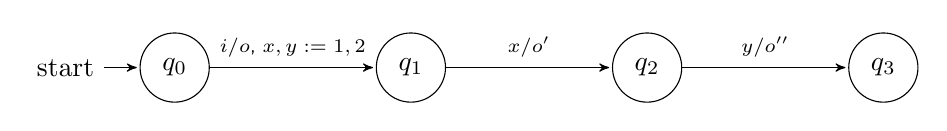
\begin{tikzpicture}[->,>=stealth',shorten >=1pt,auto,node distance=3cm,main node/.style={circle,draw,font=\sffamily\large\bfseries}]
  \node[initial, state] (1) {$q_0$};
  \node[state] (2) [right of=1] {$q_1$};
  \node[state] (3) [right of=2] {$q_2$};
  \node[state] (4) [right of=3] {$q_3$};

  \path[every node/.style={font=\sffamily\scriptsize}]
    (1) edge node {$i/o$, $x, y:=1,2$} (2)  
    (2) edge  node {$\toevent{x}/o'$} (3)
   (3) edge node {$\toevent{y}/o''$} (4);
\end{tikzpicture}

\vspace{1 em}
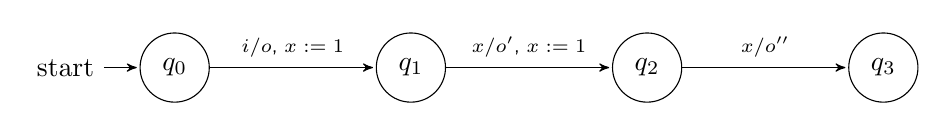
\begin{tikzpicture}[->,>=stealth',shorten >=1pt,auto,node distance=3cm,main node/.style={circle,draw,font=\sffamily\large\bfseries}]
  \node[initial, state] (1) {$q_0$};
  \node[state] (2) [right of=1] {$q_1$};
  \node[state] (3) [right of=2] {$q_2$};
  \node[state] (4) [right of=3] {$q_3$};

  \path[every node/.style={font=\sffamily\scriptsize}]
    (1) edge node {$i/o$, $x:=1$} (2)  
    (2) edge  node {$\toevent{x}/o'$, $x:=1$} (3)
   (3) edge node {$\toevent{x}/o''$} (4);
\end{tikzpicture}
\caption{Timed equivalent but not untimed equivalent}
\label{fig:twoequivalentone}
\end{center}
\end{figure}
For this reason, we will restrict ourselves in the rest of this article to MMTs in which at most
one clock can be (re)set in a single transition. This restriction has the additional advantage that it
eliminates the uncontrollable nondeterminism
of the MMTs of Figures~\ref{fig:nondeterminism} and \ref{fig:nondeterminism2}.
Provided there is no uncontrollable nondeterminism, most MMTs
have an equivalent MMT that (re)sets at most one timer per transition:
if multiple timers are started simultaneously then we can often encode this by just
starting the timer $x$ with the smallest value $d_0$, and recording the set of remaining timers in the discrete state.
Then, when $x$ expires, we start the next timer (with timeout value decremented by $d_0$), etc.
However, such an encoding is not always possible. 
Figure~\ref{fig:counterexample} presents an example of an MMT for which no equivalent MMT exists
in which at most one timer is (re)set per transition.
\begin{figure}
\begin{center}
\begin{tikzpicture}[->,>=stealth',shorten >=1pt,auto,node distance=2.7cm,main node/.style={circle,draw,font=\sffamily\large\bfseries}]
  \node[initial, state] (1) {$q_0$};
  \node[state] (2) [right of=1] {$q_1$};
  \node[state] (3) [right of=2] {$q_2$};
  \node[state] (4) [right of=3] {$q_3$};
  \node[state] (5) [below of=2] {$q_4$};

  \path[every node/.style={font=\sffamily\scriptsize}]
    (1) edge node {$i/o$, $x, y:=1,2$} (2)  
    (2) edge  node {$i/o$} (3)
   (3) edge node {$\toevent{y}/o''$} (4)
   (2) edge node {$\toevent{x}/o'$} (5);
\end{tikzpicture}
\caption{Starting more than one timer on a transition increases expressivity}
\label{fig:counterexample}
\end{center}
\end{figure}

Even when we restrict to MMTs that may (re)set at most one timer per transition, there is a difference
between the timed and the untimed semantics.
This is due to the fact that an MMT may have timers that are always stopped or restarted before
they expire. Such ``ghost'' timers are visible in the untimed semantics but cannot be observed in the timed semantics.
Figure~\ref{fig:ghosttimers} gives an example of an MMT with a ghost timer. The MMT is equivalent to the MMT obtained by 
omitting the update $y :=60$ on the transition from $q_1$ to $q_2$.
\begin{figure}
\begin{center}
\begin{tikzpicture}[->,>=stealth',shorten >=1pt,auto,node distance=2.7cm,main node/.style={circle,draw,font=\sffamily\large\bfseries}]
  \node[initial, state] (1) {$q_0$};
  \node[state] (2) [right of=1] {$q_1$};
  \node[state] (3) [right of=2] {$q_2$};
  \node[state] (4) [right of=3] {$q_3$};
  \node[state] (5) [below of=2] {$q_4$};

  \path[every node/.style={font=\sffamily\scriptsize}]
    (1) edge node {$i/o$, $x:=1$} (2)  
    (2) edge  node {$i/o$, $y:=60$} (3)
   (3) edge node {$\toevent{x}/o''$} (4)
   (2) edge node {$\toevent{x}/o'$} (5);
\end{tikzpicture}
\caption{MMT with a ghost timer $y$}
\label{fig:ghosttimers}
\end{center}
\end{figure}
%Let $\M$ be an MMT. Then we say that $\M$ is \emph{timer live} if, for each time run $\alpha$ and for each timer $x$
%\marginpar{How can we decide timer liveness?}
%of the final configuration of $\alpha$, there exists an extension $\alpha'$ of $\alpha$ in which timer $x$ 
%remains unaffected until it expires.

We say that an MMT $\M$ is \emph{timer live} if, for each feasible untimed behavior $\beta$ and for each timer $y$ that is running after $\beta$, there exists an untimed behavior $\beta_y$ consisting of transitions that leave $y$ unaffected, except for the last one in which $y$ expires, and such that $\beta \cdot \beta_y$ is feasible.
Clearly, the MMT of Figure~\ref{fig:ghosttimers} is not timer live, as there is no way to extend the feasible untimed
behavior $\emptyset \xrightarrow{i/o,~ x:=1 } \{ x\} \xrightarrow{i/o,~ y:=60 } \{ x, y\}$ to an untimed behavior in which
timer $y$ expires.

We will prove that the timed semantics and the untimed semantics coincide for timer live MMTs in which at most one timer is (re)started on each transition. However, before we can prove this result we need to do some prepatory work.

\paragraph{Wiggling}
Often it is possible to slightly change the timing of events in a timed behavior, 
while preserving the associated untimed behavior.
Clearly, if we shift the timing of an input event by a small amount then we must also shift the timing of the corresponding timeout event
by the same amount. In addition, if the timeout event starts another timer then we also need to shift the timeout event that this timer induces, etc.
%
Let us formalize these ideas. Consider a timed behavior $\sigma$ as in equation (\ref{timedbehavior}).
We say that event $i_p$ \emph{triggers} $i_q$ if $p<q$ and there exists a timer $x$ such that:
(a) event $i_p$ starts $x$, 
(b) for all $p < r < q$, $x$ is unaffected by event $i_r$, and
(c) $i_q = \toevent{x}$.
A \emph{trigger sequence} of $\sigma$ is a maximal subset of indices $T = \{ p_1 ,\ldots, p_u \}$ such that $i_{p_1} \in T$, $i_{p_1}$ triggers $i_{p_2}$, $i_{p_2}$ triggers $i_{p_3}$, etc.
The following lemma allows us to shift all the events in a trigger sequence forward and backward by a small amount, 
under the condition that all valuations are injective, that is, distinct timers have distinct values.

\begin{lemma}[Wiggle lemma]
\label{wiggle lemma}
Suppose $\sigma$ is a timed behavior as in in equation (\ref{timedbehavior}) in which all valuations
$\kappa_j, \kappa'_j$ are injective.
Suppose $T = \{ p_1 ,\ldots, p_u \}$ is a trigger sequence of $\sigma$, and suppose
that $\epsilon$ is a real number whose absolute is smaller than any nonzero number that occurs in $\sigma$, that is
$\mid \epsilon \mid  < \min (\bigcup_{1 \leq j \leq k} \{ d_j \} \cup \ranof{\kappa'_j} \setminus \{ 0 \} )$.
Then there exists a timed behavior
\begin{eqnarray*}
\sigma' & = & \lambda_0 \xrightarrow{e_1} \lambda'_0 \xrightarrow{i_1/o_1, \rho_1} \lambda_1 \xrightarrow{e_2} \lambda'_1 \xrightarrow{i_2/o_2, \rho_2} \lambda_2 \cdots
\xrightarrow{e_k} \lambda'_{k-1} \xrightarrow{i_k/o_k, \rho_k} \lambda_{k}
\end{eqnarray*}
in which all valuations are injective such that
$\untime(\sigma)=\untime(\sigma')$,
$\kappa_0 = \lambda_0$, and
\begin{eqnarray*}
e_j & = & \left\{ \begin{array}{ll}
d_j + \epsilon & \mbox{if } j-1 \not\in T \wedge j \in T \\
d_j & \mbox{if } j-1 \in T \Leftrightarrow j \in T\\
d_j - \epsilon & \mbox{if } j-1 \in T \wedge j \not\in T
\end{array}\right.
\end{eqnarray*}
\end{lemma}
The next example shows that, without the assumption of injectivity, Lemma~\ref{wiggle lemma} does not hold. 

\begin{example}
\label{no wiggling example}
Consider the following timed behavior with trigger sequences $\{ 1, 3 \}$, $\{ 2 \}$, and $\{ 4, 5 \}$:
\[
\emptyset \xrightarrow{7} \emptyset \xrightarrow{i_1/o_1, x \mapsto 2} (x=2) \xrightarrow{1} (x=1)
\xrightarrow{i_2/o_2, y \mapsto 1} (x=y=1) \xrightarrow{1} (x=y=0) 
\]
\[
\xrightarrow{\toevent{x}/o_3, u \mapsto 2} (u=2)
\xrightarrow{1} (u=1)
\xrightarrow{i_4/o_4, z \mapsto 1} (u=z=1)
\xrightarrow{1} (u=z=0)
\]
\[
\xrightarrow{\toevent{z}/o_5} (u=0).
\]
Not all valuations in this timed behavior are injective because $i_2$ sets $y$ to $1$ exactly when $x$ equals $1$,
and $i_4$ sets $z$ to $1$ exactly when $u$ equals $1$.
As a result of these ``coincidences'' we cannot wiggle the timing of trigger sequence $\{ 1, 3 \}$ by any amount:
if $i_1$ occurs just a bit later then timer $y$ must expire before timer $x$,
and if $i_1$ occurs just a bit earlier then timer $u$ must expire before timer $z$.
Note that when timer $x$ expires timer $y$ is stopped.
\end{example}

Fortunately, for any timed behavior that contains valuations that are non-injective,
an equivalent timed behavior exists in which all valuations are injective.
We may for instance slighly modify the timed behavior of Example~\ref{no wiggling example} by letting $i_2$ occur
a bit later and the trigger sequence $\{ 4, 5 \}$ a bit earlier.
Then all valuations are injective and we can wiggle the timing of event $i_1$. 

\begin{lemma}
Let $\sigma$ be any timed behavior.
Then there exists a timed behavior $\sigma'$ in which all valuations are injective such that
$\untime(\sigma)=\untime(\sigma')$.
\end{lemma}
\begin{proof}
Assume that $\sigma$ contains a valuation that is not injective. By induction on the smallest number
\end{proof}


\begin{theorem}
\label{timedimpliesuntimed}
Suppose that $\M$ and $\N$ are timer live MMTs in which at most one timer is started on each transition. Then
$\M \approx_{\mathit{timed}} \N$
implies
$\M \approx_{\mathit{untimed}} \N$.
\end{theorem}
\begin{proof}
Suppose that $\M \approx_{\mathit{timed}} \N$.
Let $\beta$ be a feasible untimed behavior of $\M$.
By induction on the number of events in $\beta$, we prove that $\N$ has a feasible untimed behavior that is isomorphic to $\beta$.
Since $\approx_{\mathit{untimed}}$ is symmetric, this suffices to prove the theorem.

Induction base. If $\beta$ contains $0$ events then it consists of the empty set of variables $\emptyset$.
Since $\emptyset$ is a feasible untimed behavior of any MMT, $\beta = \emptyset$ is a feasible untimed behavior of $\N$, as required.

Induction step. Suppose $\beta$ contains $k+1$ events:
\begin{eqnarray*}
\beta & = & X_0 \xrightarrow{i_1/o_1, \rho_1} X_1  \xrightarrow{i_2/o_2, \rho_2} X_2 \cdots \xrightarrow{i_k/o_k, \rho_k} X_{k}
 \xrightarrow{i_{k+1}/o_{k+1}, \rho_{k+1}} X_{k+1}.
\end{eqnarray*}
Let $\delta$ be the prefix of $\beta$ containing $k$ events. Then $\delta$ is also a feasible untimed behavior and thus, by
induction hypothesis, there exists an isomorphism $f = f_0 ,\ldots, f_k$ and a feasible untimed behavior
\begin{eqnarray*}
\delta' & = & Y_0 \xrightarrow{i_1/o_1, \tau_1} Y_1  \xrightarrow{i_2/o_2, \tau_2} Y_2 \cdots \xrightarrow{i_k/o_k, \tau_k} Y_{k}
\end{eqnarray*}
of $\N$ such that $\delta' = f(\delta)$.
\end{proof}

\subsection{Reachability analysis}
For any nonempty sequence $\sigma$, $\Head{\sigma}$ denotes the first element of $\sigma$, $\Tail{\sigma}$ denotes the sequence obtained by removing the first element from $\sigma$, and $\Last{\sigma}$ denotes the last element of $\sigma$.
Suppose $\beta, \beta'$ are untimed behaviors over $I$, $O$ and $Y$ such that $\Last{\beta} = \Head{\beta'}$.
Then $\beta \cdot \beta'$, the \emph{sequential composition} of $\beta$ and $\beta'$, is the untimed behavior $\beta \Tail{\beta'}$.
Behavior $\beta$ is a \emph{prefix} of untimed behavior $\gamma$ if there exists an untimed behavior $\beta'$ such that $\gamma = \beta \cdot \beta'$.

It is not difficult to translate an MMTs to a timed automaton \cite{AD94,BengtssonY03} that accepts the same timed words.
Through such a translation, verification and analysis tools for timed automata, such as Uppaal \cite{Uppaal4.0}
become available for MMTs.
MMTs are strictly less expressive than timed automata. MMTs, for instance, do not contain time deadlocks or zeno loops that
may prevent time from progressing.

MMTs have infinitely (in fact even uncountably) many configurations and it is thus necessary to use symbolic representations
for reachability analysis. Given an untimed behavior $\beta$ we want to compute its effect on a set of valuations. 
If $\beta =X_0$ and $K \subseteq\Vals{X_0}$ then we define $\Post_{\beta}(K) = K$.
If $\beta = X_0 \xrightarrow{i_1/o_1, \rho_1} X_1$ and
$K \subseteq\Vals{X_0}$ then
\begin{eqnarray*}
\Post_{\beta}(K) & = & \{ \tvals'' \in\Vals{X_1} \mid \exists \tvals \in K \exists d >0 \exists \tvals' \in\Vals{X_0} :
 \tvals \xrightarrow{d} \tvals' \xrightarrow{i_1/o_1, \rho_1} \tvals'' \}.
\end{eqnarray*}
The definition of $\Post_{\beta}(K)$ is extended inductively to arbitrary $\beta$ by 
$\Post_{\gamma \cdot \gamma'}(K) = \Post_{\gamma'} (\Post_{\gamma}(K))$, where $\gamma \cdot \gamma'$ is the decomposition of
$\beta$ into an untimed behavior $\gamma$ of length one and an untimed behavior $\gamma'$.
We write $\Post_{\beta}$ as abbreviation for $\Post_{\beta}(\Vals{\Head{\beta}})$.

For any untimed behavior $\beta$, the set $\Post_{\beta}$ can be symbolically represented and computed using a Difference Bound Matrices (DBMs)
 \cite{Di89},  as the transition predicates $\xrightarrow{d}$ and $\xrightarrow{i_1/o_1, \rho_1}$ can be easily decomposed 
into elementary operations that have been defined
on DBMs such as reset, conjunction, and delay successors \cite{BengtssonY03}.

Since emptiness of DBMs is also decidable, the following lemma allows us to compute whether or not an untimed behavior is feasible.

\begin{lemma}
Suppose $\beta$ is an untimed behavior. Then $\beta$ is feasible iff $\Post_{\beta} \neq \emptyset$.
\end{lemma}
\begin{proof}
Straightforward by induction on the length of $\beta$.
\end{proof}

The next four lemma's will be used in the following subsection.

\begin{lemma}
\label{lemma: feasibility concatenation}
Suppose $\beta, \beta'$ are untimed behaviors with
% $\Last{\beta} = \Last{\beta'} = X_1$ and 
$\Post_{\beta} = Post_{\beta'}$. Let $\gamma$ be any untimed behavior.
Then $\beta \cdot \gamma$ is feasible iff $\beta' \cdot \gamma$ is feasible.
\end{lemma}

\begin{lemma}
\label{lemma finitely many zones}
Let $\M$ be an MMT. Then the set
$\{ \Post_{\beta} \mid \beta \mbox{ is a feasible untimed behavior of } \M \}$ is finite.
\end{lemma}
\begin{proof}
All the sets $\Post_{\beta}$ can be represented using DBMs. Since an MMT only has a finite number of timers that can only be set to a finite number of integer values. Since in an MMT the values of timers can only decrease, only finitely many numbers may
appear in the DBM's that represent the sets $\Post_{\beta}$. Thus all the sets $\Post_{\beta}$ can be represented by a finite
collection of DBMs.
\end{proof}

\begin{lemma}
Suppose $\beta$ is a feasible untimed behavior and $Y \xrightarrow{i/o, \rho} Y'$ is an untimed behavior,
with $Y = \Last{\beta}$ and $i \in I$.
Then $\beta \xrightarrow{i/o, \rho} Y'$ is a feasible untimed behavior.
\end{lemma}

Let $\beta$ be a feasible untimed behavior and let $x \in X$ be a timer. Then we say that $x$ is \emph{expirable} after $\beta$
if there exists a valuation in $\Post_{\beta}$ in which $x$ is minimal.

\begin{lemma}
Suppose $\beta$ is a feasible untimed behavior and $Y \xrightarrow{\toevent{x}/o, \rho} Y'$ is an untimed behavior 
with $Y = \Last{\beta}$.
Then $x$ is expirable after $\beta$ iff $\beta \xrightarrow{\toevent{x}/o, \rho} Y'$ is feasible.
\end{lemma}

\subsection{Myhill-Nerode}  
We present a variant of the famous Myhill-Nerode theorem for MMTs.
We will use this theorem as a basis for an automata learning algorithm for MMTs.

\begin{definition}
Let $S$ be a set of feasible untimed behaviors over $I$, $O$ and $Y$. Then $S$ is
\begin{itemize}
\item
\emph{prefix closed}: $\beta \beta' \in S \Longrightarrow \beta \in S$,
\item
\emph{behavior deterministic}:
$\beta \xrightarrow{i/o_1, \rho_1} X_1 \in S \wedge \beta \xrightarrow{i/o_2, \rho_2} X_2 \in S \Longrightarrow o_1 = o_2 \wedge \rho_1 = \rho_2 \wedge X_1 = X_2$,
\item
\emph{input complete}:
$\beta \in S \wedge i \in I \Longrightarrow \exists o, \rho, Y : \beta \xrightarrow{i/o, \rho} Y \in S$,
\item
\emph{timeout complete}:
$\beta \in S \wedge x \mbox{ expirable after } \beta \Longrightarrow
\exists o, \rho, Y: \beta \xrightarrow{\toevent{x}/o, \rho} Y \in S$.
\end{itemize}
Behaviors $\beta, \beta' \in S$ are \emph{equivalent} for $S$, notation $\beta \equiv_S \beta'$, iff 
$\Post_{\beta} = \Post_{\beta'}$ and for any observation
$\gamma$ over $I$, $O$ and $Y$, $\beta \cdot \gamma \in S \Leftrightarrow \beta' \cdot \gamma \in S$.
We write $[\beta]$ to denote the equivalence class of $\beta$ with respect to $\equiv_S$.
\end{definition}

\begin{theorem}
Let $S$ be a set of feasible untimed behaviors over finite sets of inputs $I$, outputs $O$, and timers $Y$.
Then $S$ is the set of feasible untimed behaviors of an MMT $\M$ iff $S$ is nonempty, all untimed behaviors in $S$
start with the empty set of timers, $S$ is prefix closed, behavior deterministic, input complete, timeout complete,
and $\equiv_S$ has only finitely many equivalence classes (finite index).
\end{theorem}
\begin{proof}

``$\Rightarrow$'' Let $\M$ be an MMT and let $S$ be the set of its feasible untimed behaviors.
Then it is immediate from the definitions that $S$ is nonempty, all untimed behaviors in $S$
start with the empty set of timers, $S$ is prefix closed, behavior deterministic, input complete, and timeout complete.
Suppose that feasible untimed behaviors $\beta$ and $\beta'$ lead to the same state $q$ and moreover $\Post_{\beta} = \Post_{\beta'}$.
Then, 
by Lemma~\ref{lemma: feasibility concatenation},
for any untimed behavior $\gamma$, $\beta \cdot \gamma \in S \Leftrightarrow \beta' \cdot \gamma \in S$, and thus
$\beta \equiv_S \beta'$.
Since $\M$ only has finitely many states and by Lemma~\ref{lemma finitely many zones} the set
$\{ \Post_{\beta} \mid \beta \mbox{ is a feasible untimed behavior of } \M \}$ is finite, this means that
$\equiv_S$ has finite index.

``$\Leftarrow$'' Suppose $S$ is nonempty, etc.
We define MMT $\M = (I, O, Q, q_0, \vars, \delta, \lambda, \remap)$ as follows:
\begin{itemize}
\item
$Q$ is the set of equivalence classes of $\equiv_S$,
\item
$q_0 = [\emptyset]$. (Note that $\emptyset \in S$ since $S$ is nonempty, prefix closed, and all untimed behaviors in $S$ start
with the empty set of timers.)
\item
$\varsof{[\beta]} = \Last{\beta}$.
\item
Let $\beta \in S$ and $i \in I$. Then, since $S$ is both input complete and behavior deterministic, there exist unique
$o$, $\rho$ and $Y$ such that $\beta' = \beta \xrightarrow{i/o, \rho} Y \in S$.
We define $\delta([\beta],i) = [\beta']$, $\lambda([\beta],i) = o$, and $\remap([\beta],i) = \rho$.
\item
Assume $\beta \in S$ and $x\in \Last{\beta}$ expirable after $\beta$. 
Then, since $S$ is both input complete and behavior deterministic, there exist unique
$o$, $\rho$ and $Y$ such that $\beta' = \beta \xrightarrow{\toevent{x}/o, \rho} Y \in S$.
We define $\delta([\beta],\toevent{x}) = [\beta']$, $\lambda([\beta],\toevent{x}) = o$, and $\remap([\beta],\toevent{x}) = \rho$.
\item
Assume $\beta \in S$ and $x \in \Last{\beta}$ not expirable after $\beta$.
We define $\delta([\beta],\toevent{x}) = [\beta]$, $\lambda([\beta],\toevent{x}) = \Lambda$, and $\remap([\beta],\toevent{x}) = \rho_0$, where $\domof{\rho_0} = \emptyset$.
\end{itemize}
It is routine to verify that $M$ is a well-defined MMT whose set of feasible untimed behaviors equals $S$.
\end{proof}



\section{Automata Learning for MMTs}
In this section, we present an algorithm for automata learning for MMTs.
It is based on the Nerode equivalence $\equiv_{\M}$, which is used to adapt
the standard paradigm for automata learing, using $L^*$, which is also adapted
to register automata in~\cite{CasselHJS16}. 

Thus, two tasks must be accomplised in order to design the algorithm.
\begin{itemize}
  \item
    One task is to infer untimed traces of am MMT.
    This is done by supplying membership queries, in the form of inputs
    with specific timing.
\item
  One task is to define suitable approximations of $\equiv_\M$, which are
  based on finite sets of suffixes. We must determine how to define suitable
  finite sets of suffix traces, which are used to define overapproximations
  of $\equiv_\M$.
\end{itemize}
We assume that we can observe
exact timing of events and that we can observe whenever a timeout event
happens. We cannot directly observe the setting of timers, or the identity
of the timer in a timeout event. However, whenever a timeout event, we
can infer where it was set, by supplying a small sequence of membership queries
with slightly perturbed timing. This is a consequence of the fact that we
assume MMTs to be robust, implying that we can always include ``slack'' in
the timing of inputs. The normalized name of the timer follows after inferring
in which transition it was set.

Let us begin with the second task.
Intuitively, we are looking for a mechanism for characterizing a finite
set of suffixes, so that we can adapt the definition of
$\uttrace \equiv^{\timerequiv} \uttrace'$ to consider specific subsets of
suffixes. The natural way to do this is, like~\cite{Nie03}, to define
finite sets of input sequences. In our setting, a complication is that
input sequences include timer events, of form $\toevent{x}$, and that
after different traces, timer events with different timers may or may
not be enabled. We solve this complication by omitting the
identity of the timer $x$ in input sequences that characterize suffixes.

Let an \emph{input prefix} be a sequence of extended inputs.
For a trace $\uttrace$, let $\pinpof{\uttrace}$ be the sequence of its
inputs an timer events.
Let a \emph{timeout symbol} be of form $\tosymbol$, i.e., a
timer event without any clock.
Let an \emph{input suffix} be a sequence of inputs and timeout symbols.
For a suffix trace $\strace$, let $\sinpof{\strace}$ be the sequence
of inputs and timeout symbols in $\strace$, i.e., $\sinpof{\strace}$ is the
sequence of extended inputs, but with timers removed from timer events.

A central mechanism in our active learning algorithm is a procedure which
takes  an input prefix $u$ and an input suffix $v$ and return the set of
untimed traces of form $\uttrace\conc\strace$ such that
$\pinpof{\uttrace} = u$ and $\sinpof{\strace} = v$. We must here take into
consideration that we may not be able to observe all timer settings of the
SUT; only those timer settings that can actually expire sometime during
$\uttrace\conc\strace$ can actually be observed.
This may further depend on the timing of transitions
in $\uttrace\conc\strace$.

%% Let us now consider the issue that timeout events are not always
%% enabled.
%% Consider a trace $u$ of $\M$, and assume that timer $x$ is set in the
%% $i$th event of $u$. Then, in each state the corresponding timeout even
%% $\toevent{x}$ may or may not be enabled; this may
%% further depend on the timing of events in $u$, including
%% the timing of events that precede the $i$th event.
%% This motivates the following definitions.

Motivated by these considerations,
let $\uttrace = \tuple{i_1,o_1,\remapinst_1}\cdots\tuple{i_n,o_n,\remapinst_n}$.
We say that $\uttrace$ is {\em feasible} if 
there is a corresponding timed word
$\tword = (i_1, o_1, t_1) \cdots (i_n, o_n, t_n)$ for some $\vect tn$.
We then say that $\tword$ is {\em derived} from $\uttrace$.
Let $\expirable(\uttrace)$ be the set of timers $x$ such that
$\tuple{i_1,o_1,\remapinst_1}\cdots\tuple{i_n,o_n,\remapinst_n}
\tuple{\toevent{x},o_{n+1},\remapinst_{n+1}}$
is feasible for some $o_{n+1}$, $\remapinst_{n+1}$.
For $u = \pinpof{\uttrace}$ we say that $u$ is feasible iff $\uttrace$ is
feasible, and define $\expirable(u) = \expirable(\uttrace)$.

%% For a sequence $u = i_1 \cdots i_n$, define $\uttraceof{u}$ as the normalized
%% trace $\tuple{i_1,o_1,\remapinst_1}\cdots\tuple{i_n,o_n,\remapinst_n}$
%% if it exists, otherwise $\uttraceof{u} = \bot$. We say that $u$ is {\em feasible}
%% if $\uttraceof{u}$ is defined and is feasible. Define
%% $\expirable(u)$ to be $\expirable(\uttraceof{u})$.
%% It follows that $u = i_1 \cdots i_n$ is feasible if and only if whenever
%% $i_k$ is a timeout event $\toevent{x}$ for some $k$ with $1 < k \leq n$, then
%% $x \in \expirable(i_1 \cdots i_{k-1})$.
%% We will later present a technique for inferring the set $\expirable(u)$.

\paragraph{Membership Queries}
The procedure for inferring untimed traces will utilize membership queries.
We will slightly adapt the notion of membership query to make it convenient
in our current setting.

A {\em membership query} is an alternating sequence
$t_1i_2t_2i_2 \cdots t_ni_nt_{n+1}$ of delays and inputs in $\extinputs$.
The response to a membership query is either
\begin{itemize}
\item
  a sequence $o_1 o_2 \cdots o_n$ of outputs in $O$, meaning that there is
  a corresponding timed word $(i_1, o_1, t_1) \cdots (i_n, o_n, t_n)(i_{n+1}, o_{n+1}, t_{n+1})$ for some $i_{n+1}$, $o_{n+1}$, $t_{n+1}'$ with $t_{n+1} \leq t_{n+1}'$,
  or
\item
  a timeout event after some prefix $t_1i_2t_2i_2 \cdots t_{k-1}i_{k-1}t_{k}'$
  where $k \leq n+1$ and $t_k' \leq t_k$, implying that  there is
  a corresonding timed word $(i_1, o_1, t_1) \cdots (\toevent{x}, o_k, t_k')$
  for some timer $x$. By the assumption of robustness, it is easy to
  determine where the timer $x$ was set. Therefore the response to the
  membership query is the index $k$ and the normalized timer name
  $\timerof jp$, or
\item
  a {\em missing timer event} after some prefix
  $t_1i_2t_2i_2 \cdots t_{k-1}i_{k-1}t_{k}$, implying that input $i_k$, of
  form $\toevent{x}$, does not occur at the intended time.
\end{itemize}

\paragraph{Inferring traces}
We can now present a central procedure of our learning algorithm,
which is one that 
takes a feasible input prefix $u$ and an input suffix $v$ and returns the set of
feasible (normalized) untimed traces of form $\uttrace\conc\strace$ such that
$\pinpof{\uttrace} = u$ and $\sinpof{\strace} = v$.
%% restricted to the set of timers that are in
%% $\expirable(i_1 \cdots i_{k})$ for some $k \leq n$.
We assume that names of timers are normalized.

%% Consider a trace 
%% $\tuple{i_1,o_1,\remapinst_1}\cdots\tuple{i_n,o_n,\remapinst_n}$.
%% and let 
%% $w = (i_1, o_1, t_1) \cdots (i_n, o_n, t_n)$ be a corresonding timed word.
%% We introduce the following canonical naming convention for timers.
%% A timer which is set to $p$ at transition $j$ (i.e., in response to
%% input $i_j$ is given the name $\timerof jp$. This means that
%% for a timer $\timerof jp$ we have
%% $\remapinst_j(\timerof jp) = p$, and that 
%% $\timerof jp \in \remapinst_k$ only if $j \leq k$ and $\timerof jp$ has
%% not expired at or before $i_k$, and then 
%% $\remapinst_k(\timerof jp) = \timerof jp$ if $j < k$.
%% We also extend $w$ by a delay $t_{n+1} \in \realsplus$, which intuitively
%% represents that time $t_{n+1}$ elapses after the trace; such a delay
%% may be observed only if it is not interrupted by a timeout event.


%% For each timer setting in the trace, i.e., each occurrence of
%% a timer  $x \in \domof{\remapinst_i}$ with  $\remapinst_i(x) \in \natplus$,
%% defined the constraint $\constrof{\word}$ as
%% \begin{itemize}
%% \item
%%   if $i_k$ is the timeout event $\toevent{x}$, then
%%   $\constrof{\word}$ is $\delay{i}{k}= \remapinst_i(x)$,
%% \item
%%   if the trace includes no timeout event $\toevent{x}$, then
%%   $\constrof{\word}$ is $\delay{i}{(n+1)} \leq \remapinst_i(x)$.
%% \end{itemize}
%% Define $\constrof{\word}$ as
%% the conjunction of $\constrof{\word}$ for all timer settings in the trace.

The procedure must find all ways to instantiate the timeout symbols in $v$
with actual timers to obtain a feasible instantiation of $u\conc v$, and for
each such instantiation determine the set of timers that may expire after some
prefix, and how they are manipulated.

Our procedure considers increasing prefixes $z$ of extended inputs that
instantiate some prefix of $u \conc v$. For each such prefix, it
determines the set $\expirable(z)$, the constraint $\constrof{z}$
under which $z$ can be performed without any succeeding timer event, 
the timers that are in $\expirable(z')$ for some prefix $z'$ of $z$, and
their manipulation.

The procedure performs repeated membership queries for selected values
of $\vect{t}{n+1}$, and gradually adds new timers to the word together
with constraints on $\vect{t}{n+1}$ induced by these timers.

Let $\delay{j}{k}$ denote $t_{j+1} + t_{j+2} + \cdots + t_k$.
%% This means that $\remapinst_j(\timerof jp) = p$, and that 
%% $\remapinst_l(\timerof jp) = \timerof jp$ if $j < l < k$.
%% This means that $\timerof jp \in \domof{\remapinst_l}$ iff
%% $j \leq l < k$, where $\remapinst_j(\timerof jp) = p$ and
%% $\remapinst_l(\timerof jp) = \timerof jp$ for $j < l < k$.
%% Initially, $\constrof{\word}$ is the conjunction of the constraints of form
%% $\delay{j}{k}=m$ for each $i_k$ of form is $\toevent{\timerof jp}$.

%% The procedure considers prefixes in increasing order. For each input prefix
%% $z$, it
%% \begin{itemize}
%% \item determines all timers that are in $\expirable(z)$,
%% \item gradually builds a constraint $\constrof{z}$ under which $z$ can
%%   be performed without interruption by unexpected timer events,
%% \item
%%   gradually builds the mappings $\remapinst_{z'}$ for prefixes $z'$ of $z$.
%% \end{itemize}

\medskip
\noindent{\bf Algorithm} \textsl{Infer-Traces.}
\begin{description}
\item[Input:] (normalized) feasible input prefix $u$ and input suffix $v$,
\item[Returns:] set of (normalized) traces
$\uttrace\conc\strace$ such that
$\pinpof{\uttrace} = u$ and $\sinpof{\strace} = v$, together with
  constraint $\constrof{\uttrace\conc\strace}$ on derived timed words.
\item[Initialization:]
    Let $z = \emptyword$, let $\constrof{z} = \true$;
\item[Return:]
    $\textsc{Infer-Traces}(\emptyword,\emptyword,\true)$
%%     \begin{itemize}
%% \item initialize $\vect{\remapinst}n$ by letting
%%     $\timerof jp \in \domof{\remapinst_l}$ iff $i_k$ is $\toevent{\timerof jp}$
%%     with $j \leq l < k$; let $\remapinst_j(\timerof jp) = p$ and
%%     $\remapinst_l(\timerof jp) = \timerof jp$ for $j < l < k$;
%% \item let $\constrof{\uttrace}$ be
%%     the conjunction of the constraints of form
%% $\delay{j}{k}=p$ for each $i_k$ of form $\toevent{\timerof jp}$.
%%     \end{itemize}
\end{description}
\medskip
\noindent{\bf Function} $\textsc{Infer-Traces}(z,\uttrace,\constrof{\uttrace})$;
\begin{enumerate}
\item
  let $z = i_1 \cdots i_m$;
  let $\uttrace = \tuple{i_1,o_1,\remapinst_1}\cdots\tuple{i_m,o_m,\remapinst_m}$;
\item
  {\bf for} each index $k = 1, \ldots , m$ {\bf do}:
     \qquad \textit{// find all timers in $\expirable(z)$}
  \begin{enumerate}
  \item
    find $\vect t{{m+1}}$ that maximizes $\delay{k}{(m+1)}$ given
    $\constrof{\uttrace}$;
  \item
    supply membership query $t_1i_2t_2i_2 \cdots t_mi_mt_{m+1}$;
  \item
    {\bf if} unexpected timeout $\toevent{\timerof jp}$ occurs within at most
    $t_{m+1}$ after $i_m$:
    \begin{enumerate}
    \item
      add $\timerof jp$ to $\domof{\remapinst_l}$ iff
$j \leq l \leq m$, where $\remapinst_j(\timerof jp) = p$ and
      $\remapinst_l(\timerof jp) = \timerof jp$ for $j < l \leq m$;
    \item
      Add conjunct 
      $\delay{j}{(m+1)} \leq p$ to $\constrof{\uttrace}$;
      \todobj{should it be $\delay{j}{(m+1)} < p$?}
    \item if $k \neq j$ go to (a);
    \end{enumerate}
    {\bf else} do nothing;
  \end{enumerate}
  {\bf od}
\item
  {\bf if} $\lengthof{z} = \lengthof{u} + \lengthof{v}$ {\bf return}
  $\tuple{\uttrace,\constrof{\uttrace}}$;
\item
  {\bf if} $i_{m+1} \in \extinputs$:
  \[  \textbf{return } \textsc{Infer-Traces}(zi_{m+1},\uttrace\tuple{i_{m+1},o_{m+1},\emptyset},\phi')
  \]
  where $\phi'$ is $\constrof{\uttrace}$ if $i_{m+1} \in I$, otherwise, if
  $i_{m+1} = \toevent{\timerof jp}$, it is obtained from $\constrof{\uttrace}$
  by replacing $\delay{j}{(m+1)} \leq p$ by $\delay{j}{(m+1)} = p$.
  \item
  {\bf else} \hspace*{4cm} \textit{// \ $i_{m+1}$ is the timeout symbol}
    \[
    \textbf{return} \mathop\bigcup_{\timerof jp \in \expirable(z)}
     \textsc{Infer-Traces}(z\toevent{\timerof jp},\uttrace\tuple{\toevent{\timerof jp},o_{m+1},\emptyset},\phi')
     \]
  where  $\phi_j^p$ is obtained from $\constrof{\uttrace}$
  by replacing $\delay{j}{(m+1)} \leq p$ by $\delay{j}{(m+1)} = p$.
\end{enumerate}
Intuitively, the function
$\textsc{Infer-Traces}(z,\uttrace,\constrof{\uttrace})$ finds
all timers in $\expirable(z)$ by testing for each $k$ whether 
it is possible
to set a timer at the $k$th transition that may expire after the
$m$th transition. Any such timer expiration adds a constraint to
$\constrof{\uttrace}$, which is included in the constraints used to find
further timers.
This is done by finding a timed word is found which maximises the
time within which it is able to expire, subject to the constraints under
which other, already detected, timers cannot expire. If no expiration is
observed, then it is ascertained that no such timer exists.
If such a timer may exist, then some expiration must be observed, either
by a timer set at the $k$th transition and expiring at the $m+1$st transition,
or by a so-far undetected timer that can expire because the membership
query exposes a new timing pattern. In either case, the new detected timer
is added to the word, and the procedure restarts.

\paragraph{Generating MMTs}
Having solved the problem of inferring untimed traces, we can now
define our generalization of $L^*$, which is based on the
Nerode equivalence defined earlier
%% We can now present our algorithm for active learning of MMTs.
%% The main structure of the algorithm is inherited from other active
%% algorithms: it builds on a Nerode equivalence, which is defined based on
%% the set of (untimed) traces of an MMT.
%% Thus, the algorithm has two nontrivial parts.
%% \begin{itemize}
%%   \item
%%     One part is to infer untimed traces of am MMT, essentially building
%%     a prefix tree of untimed traces. This is done by supplying membership
%%     queries, following the ideas of the previous section.
%% \item
%%   One part is to ``fold'' the prefix tree developed in the first part
%%   into a MMnt. This can be done by adapting the suitable tools for active
%%   automata learning, as found in $L^*$
%%   (adapted for Mealy machines in~\cite{Nie03} and to automata with
%%   data registers in~\cite{CasselHJS16}).
%% \end{itemize}
%% We assume that we can observe
%% exact timing of events and that we can observe whenever a timeout eMMvent
%% happens. On the other hand, we cannot observe the setting and resetting of
%% timers, and we cannot observe which timer caused an observed timeout event.


\begin{definition}[Observation Table]
  An \emph{observation table} is a tuple
  $\tuple{U,U^+,V,\smap}$, where
  \begin{itemize}
  \item $U$ is a set of (feasible) {\em input prefixes},
  \item $U^+$ is a set of {\em extended input prefixes}, each of form $ui$ for
    $i \in \extinputs$ (note that $U^+$ is in general not disjoint from $U$),
  \item
    $V$ is a set of input suffixes,
  \item
    $\smap$ maps each extended input prefix $u$ in $U^+$ and input suffix $v$
    to a set of pairs $\tuple{\uttrace,\strace}$ such that 
    $\uttrace\conc\strace$ is an untimed trace with
$\pinpof{\uttrace} = u$ and $\sinpof{\strace} = v$.
   We use $\smappre(u,v)$ for $\uttrace$ and 
   $\smapsuf(u,v)$ for $\strace$.
  \end{itemize}
\end{definition}
For an observation table and $u \in U^+$,
let $\obspre(u)$ denote
\(
\displaystyle\mathop\sqcup_{v \in V}\smappre(u,v)
\),
i.e., $\obspre(u)$ includes manipulation of all timers that may be
exposed by any of the suffixes in $V$.
The observation table defines the following equivalence
Let $u \equiv_{\smap}^{\timerequiv} u'$ denote that
$\timerequiv: \domof{\obspre(u)} \rightarrow \domof{\obspre(u')}$
is a bijection such that there is a bijection $\timerbij$ on $X$ with
$\timerequiv \extendedby\timerbij$ such that for each $v \in V$
\[
\strace \in \smapsuf(u,v)
\qquad \mbox{if and only if} \qquad
\timerequiv(\strace) \in \smapsuf(u',v)
\]
Let $u \equiv_{\smap} u'$ denote that 
$u \equiv_{\smap}^{\timerequiv} u'$ for some bijection
$\timerequiv: \domof{\obspre(u)} \rightarrow \domof{\obspre(u')}$.

Say that an observation table is {\em closed} if for each
$ui \in U^+$ there is a short prefix $u' \in U$ and a $\timerbij$ such that
$ui \equiv_{\smap}^{\timerequiv} u'$.

A closed observation table $\tuple{U,U^+,V,\smap}$ can be used to construct
a hypothesis  MMT $\M = (I, O, Q, q_0, \vars, \delta, \lambda, \remap)$, where
\begin{itemize}
\item
  $Q = U$ and $q_0 = \emptyword$,
\item
  $\vars$ maps each state $u \in Q$ to $\domof{\obspre(u)}$,
\item
  $\delta(u,i)$ is the unique short prefix $u'$ such that
  $ui \equiv_{\smap}^{\timerequiv} u'$. If so, then
  $\remap(u,i) = \remap\circ\timerequiv^{-1}$,
  where $\remap$ is the remapping of the last transition in
  $\obspre(ui)$.
  \item
$\lambda$ is obtained easily from the work (To be done)
\end{itemize}










%% \input{../OldFiles/oldstuff-bj-nclocks}
%% \input{textbank}
%\section{Learning algorithm}
In order to learn a MMTO, we may adapt a standard algorithm for learning (untimed) Mealy machines, e.g., $L^\ast$.
We assume that the learner knows an upper bound $B$ on the possible timeout values, that is, a constant $B \in \nat$ such
that, for each $q \in Q$, $\tau(q) < \infty$ implies $\tau(q) < B$.
Whenever we discover a new state, that is, a prefix $\beta$ of inputs that uniquely determines a state in the MMTO,
we may figure out the corresponding value of the timeout function as follows: by taking transitions in $\beta$ as
fast as possible, we ensure that the value of the timer is $0$ upon arrival in the state.
Now we just wait for $B$ time units. If an event occurs before the $B$ time units have elapsed, we record the delay after
which this event occurs: this is the value of the timeout function for state $\beta$.
Otherwise, if no event occurs and $B$ time units have elapsed, we know the value of the timeout function is $\infty$.
We record the observed value of the timeout function in a separate column in the observation table.
(Or, equivalently, we may annotate the output in the column for suffix $\mathit{to}$ with this value.)
Now suppose we have found a state that can be reached by a prefix $\beta$, and we want to figure out
whether the timer is reset after some input $i$.
We can do this as follows.
First we perform all the inputs from $\beta$ as fast as possible, ensuring that the value of the timer is $0$ in
the resulting state.
Now we wait $0.5$ time units.
If a timeout has occurred during this interval then we know that the timeout value of the state after $\beta$ is $0$.
Thus input $i$ may only occur at time $0$ and it does not make any difference whether or not the timer is reset as part
of an $i$-transition.
If no timeout occurs during the $0.5$ time units, then we perform the input $i$ and wait for $B$ time units.
If no timeout occurs during this interval then we conclude that the timer is switched of after trace $\beta \; i$,
and again it does not make a difference whether or not the timer is reset as part of the $i$-transition.
If, however, a timeout occurs $t$ time units after the input $i$, then there are two cases:
\begin{enumerate}
\item
$t$ is equal to the value of the timeout function for trace $\beta \; i$, and we may conclude that
the timer is reset as part of the $i$-transition, or 
\item
$t$ is equal to the value of the timeout function for trace $\beta \; i$ \emph{minus} $0.5$, and
we may conclude that the timer is not reset in the $i$-transition.
\end{enumerate}
We record the observed value of the reset function in the observation table in the entry for row $\beta$ and
column $i$.

The above algorithm can be implemented as a minor adaptation of existing implementations of $L^{\ast}$. The query
complexity is the same as that of $L^{\ast}$. The total time of running a query will be at most $(u+1) \cdot B + 0.5$,
where $u$ is the number of \emph{to} inputs that occur in the query.

\paragraph{Research questions}
Work out the proofs. What is the best/easiest way to implement this?
Does it also work for register automata.
Can we generalize these ideas to richer classes of automata (e.g. more clocks, splitting inputs and outputs into separate
transitions, closure under composition)?
Implement and apply this stuf, for instance to the TCP protocol.
\ifshort
\vspace{-1em}
\fi
\section{Conclusions and Future Work}
\label{conclusions}

We have presented a new automaton-based model for timed systems, MMTs,
which aims to
be sufficiently simple to allow tractable learning algorithms, and sufficiently
expressive to model common network protocols. For the MMT model we have
developed a Nerode congruence, allowing to define canonical forms, and used it
as the basis for an active learning algorithm, which generalizes $L^*$.
A key technical result is to show the equivalence between the timed semantics,
which is suitable to represent practical learning scenarios, and the
untimed semantics, which is suitable for formulating automata learning
algorithms. This equivalence is embodied by an adaptor, which transforms
queries in one model to queries in the other.

The query complexity of our learning algorithm is polynomial in the number of
states of the learned MMT, but doubly exponential in the number of simultaneously
active timers. Since practical network protocols have at most a couple of
simultaneously active timers, this leads us to believe that our work will
be a suitable theoretical basis for practical learning algorithms for such
protocols, and similar classes of timed systems.

%% Our work consitutes a major step towards a practical approach for active learning of timed systems.
%% Such an approach would greatly enhance the applicability of active learning for reverse engineering of models of
%% software and hardware systems.
Future work includes to implement equivalence queries for MMTs.
In the untimed case, equivalence queries for Mealy machines are approximated using conformance testing algorithms,
for which a rich theory exists \cite{LeeY96}.
Our equivalence result between timed and untimed semantics may help to
lift such algorithms to the setting of MMTs.
A challenge is also to deal with the timing uncertainties that occur in real applications due to nondeterminism of
implementations and imprecise measurements. In a realistic
setting we may need more than one experiment to figure out which event causes a timeout. We may observe, for instance,
that slight changes in the timing of certain inputs lead to corresponding changes in the timing of certain timeouts.

%% Nevertheless, there are still major challenges that need to be addressed.
%% %
%% A first challenge is to implement equivalence queries for MMTs.
%% In the untimed case, equivalence queries for Mealy machines are approximated using conformance testing algorithms,
%% for which a rich theory exists \cite{LeeY96}.
%% We hope that our equivalence result for the timed and untimed semantics will help to lift existing conformance
%% testing algorithms to the setting of MMTs. For MMTs with a single timer this is easy, but we do not yet have good
%% conformance testing algorithms for MMTs with multiple timers.
%% %
%% A second challenge is to deal with the timing uncertainties that occur in real applications due to nondeterminism of
%% implementations and imprecise measurements. In the idealized setting of this paper we are able to
%% identify the triggering event for each timeout by providing inputs at different fractional times. In a realistic
%% setting we may need more than one experiment to figure out which event causes a timeout. We may observe, for instance,
%% that slight changes in the timing of certain inputs lead to corresponding changes in the timing of certain timeouts.
%
%% A third important challenge is to implement our algorithm and to apply it to practical case studies. In particular,
%% it is interesting to see how we can implement lookahead queries. For MMTs with a single timer this is trivial 
%% if we assume an upper bound $t$ on the value of timers (just  wait for $t+1$ time units).
%% But we still do not know whether we can always come up with efficient implementations of the lookahead oracle for applications with multiple timers.

%% \iflong
%% Just like the theory of timed automata \cite{AD94} paved the way to extend untimed model checking tools to a timed
%% setting, we hope that our work on MMTs will make it possible to lift untimed model learning tools to a timed setting.
%% MMTs can be viewed as a restricted subclass of timed automata in which clocks run backward instead of forward.
%% Many theoretical questions about MMTs, such as the complexity of equivalence checking and model checking, are still open.
%% \fi


\bibliographystyle{plain}
\bibliography{abbreviations,dbase}

\end{document}
